\documentclass[preprint,11pt]{elsarticle}

\usepackage{graphicx}
\usepackage{hyperref}
\hypersetup{
    colorlinks=true,
    citecolor=blue,
    linkcolor=black,
    urlcolor=blue,
    pdfborder={0 0 0}
}
\usepackage{tabularx}
\usepackage{pdflscape}   % Para modo paisagem
\usepackage{booktabs}    % Para \toprule, \midrule, \bottomrule
% \usepackage{geometry}    % Para ajustar margens
\usepackage{array}       % Para controle de colunas
\usepackage{adjustbox}
\usepackage{verbatim}
\usepackage{amssymb}
\usepackage{lineno}
\usepackage{amsthm}
\usepackage{graphicx}
% \usepackage{caption}
\usepackage{subcaption}
\usepackage[margin=1in]{geometry}
\usepackage{amsmath}
\usepackage{dsfont}
\usepackage{mathtools}
\usepackage{url}
\usepackage{float}
\usepackage{multirow}
\usepackage{natbib}
\usepackage{color}
\biboptions{sort&compress}
\restylefloat{table}
\usepackage{upgreek}
\usepackage{nicefrac}
\usepackage{xargs}                      
\usepackage[pdftex,dvipsnames]{xcolor} 
\usepackage[colorinlistoftodos,prependcaption,textsize=tiny]{todonotes}
%\usepackage{algorithmic}
\usepackage{xcolor}
\usepackage{multicol}
% \usepackage{algorithm}
%\usepackage[noend]{algpseudocode}
\newtheorem{theorem}{Theorem}[section]
\newtheorem{corollary}{Corollary}[theorem]
\newtheorem{lemma}[theorem]{Lemma}
\usepackage{algorithm}
\usepackage{algorithmic}
\makeatletter
%\def\BState{\State\hskip-\ALG@thistlm}
\usepackage{lipsum}
\makeatother
\usepackage{nomencl}
\makenomenclature
\renewcommand{\vec}[1]{\mathbf{#1}}
\DeclareMathOperator*{\argmax}{arg\,max}
\DeclareMathOperator*{\argminB}{arg\,min}

\theoremstyle{plain}
\newtheorem{thm}{Theorem}[section]
\newtheorem{lem}[thm]{Lemma}
\newtheorem{prop}[thm]{Proposition}
\newtheorem*{cor}{Corollary}

\theoremstyle{definition}
\newtheorem{defn}{Definition}[section]
\newtheorem{conj}{Conjecture}[section]
\newtheorem{exmp}{Example}[section]

\theoremstyle{remark}
\newtheorem*{rem}{Remark}
\newtheorem*{note}{Note}


\newcommandx{\unsure}[2][1=]{\todo[linecolor=red,backgroundcolor=red!25,bordercolor=red,#1]{#2}}
\newcommandx{\change}[2][1=]{\todo[linecolor=red,backgroundcolor=red!25,bordercolor=red,#1]{#2}}
\newcommandx{\info}[2][1=]{\todo[linecolor=OliveGreen,backgroundcolor=OliveGreen!25,bordercolor=OliveGreen,#1]{#2}}
\newcommandx{\improvement}[2][1=]{\todo[linecolor=Plum,backgroundcolor=Plum!25,bordercolor=Plum,#1]{#2}}
\newcommandx{\thiswillnotshow}[2][1=]{\todo[disable,#1]{#2}}

\usepackage{lineno}

\journal{Life Cycle Reliability and Safety Engineering}

\usepackage{tikz} %Para desenhar imagem
\usetikzlibrary{arrows.meta}


\usepackage{titlesec}

\titleclass{\subsubsubsection}{straight}[\subsubsection]
\newcounter{subsubsubsection}[subsubsection]

\renewcommand\thesubsubsubsection{\thesubsubsection.\arabic{subsubsubsection}.}

\titleformat{\subsubsubsection}
  {\normalfont\normalsize\itshape} % mesma fonte do texto + itálico
  {\thesubsubsubsection}
  {1em}
  {}

\titlespacing*{\subsubsubsection}
  {0pt}
  {3ex plus 1ex minus .2ex}
  {0.5ex plus .1ex}

\setcounter{secnumdepth}{4}
\setcounter{tocdepth}{4}
\usepackage{indentfirst}

\begin{document}

\begin{frontmatter}

\title{Modelagem paramétrica para projeto inteligente e automatizado de fundações superficiais do tipo sapata: Pré dimensionamento, projeto automatizado e confiabilidade}

\author[label1]{Filipe Amaral Pereira}
\author[label1]{Wanderlei M. Pereira Junior}
\author[label2]{  }
\author[label3]{  }
\author[label4]{Lucas Teixeira Correia}

\address[label1]{Federal University of Catalão, Engineering College, Av. Dr. Lamartine Pinto de Avelar, 1120, Catalão, 75704-020, Brazil}
\address[label2]{University of São Paulo – School of Engineering of São Carlos, Av. Trabalhador São Carlense, 400 – Parque Arnold Schimidt, São Carlos – SP, 13566-590, Brazil}
\address[label3]{Federal University of Goiás – School of Civil and Environmental Engineering, Avenida Universitária, Quadra 86, Lote Área 1488 – Setor Leste Universitário, Goiânia – GO, 74605-220, Brazil}
\address[label4]{Pontifical Catholic University of Goiás – School of Engineering, Avenida Universitária, 1440 – Setor Universitário, Goiânia – GO, 74605-010, Brazil}


\begin{abstract}
O dimensionamento de fundações superficiais do tipo sapata isolada é predominantemente realizado por procedimentos iterativos baseados na experiência do projetista, resultando frequentemente em soluções conservadoras e, consequentemente, em elevado consumo de materiais. Este artigo apresenta uma metodologia computacional que integra critérios estruturais, geotécnicos e geométricos em um único ambiente de projeto para o dimensionamento automatizado e otimizado de sapatas isoladas. A formulação adota, como função objetivo, a minimização do volume de concreto, sujeita a restrições baseadas nas normas brasileiras NBR 6118 e NBR 6122, que abrangem tensões no solo, punção, compatibilidade geométrica entre o pilar e a sapata, e sobreposição entre elementos de fundação. O problema de otimização mono-objetivo é resolvido por meio do método Efficient Global Optimization (EGO), que combina um modelo substituto baseado em regressão por processos gaussianos (\textit{Kriging}) com uma função de aquisição (\textit{Expected Improvement}) para equilibrar exploração e intensificação da busca. Um algoritmo genético (AG) é empregado como otimizador interno para maximizar a função de aquisição. A metodologia foi implementada em uma plataforma \textit{web} (\textsc{FundaAI}) e aplicada a diferentes exemplos de projetos com um, dois e três elementos de fundação. Os resultados do trabalho demonstraram que o EGO é capaz de convergir para soluções viáveis, mesmo com o aumento da dimensionalidade do problema. A ferramenta proposta alcançou reduções médias de 40,79\% no volume de concreto em comparação com simulações de Monte Carlo, que foram aplicadas para representar práticas tradicionais de tentativa e erro de escritórios, atingindo até 85,87\% em casos específicos. Através da análise das razões solicitação/resistência, foi possível identificar as restrições governantes em cada configuração, evidenciando que a otimização global pode levar a soluções nas quais nem todos os elementos atingem seus limites individuais. Em situações com alto grau de proximidade entre sapatas, a verificação de sobreposição mostrou-se eficiente na identificação, embora a metodologia atual seja mais adequada a arranjos sem interferências severas. Conclui-se que a ferramenta desenvolvida tem potencial para se tornar uma alternativa eficaz para o projeto racional de fundações, contribuindo para a redução do consumo de materiais, a diminuição dos impactos ambientais associados, a padronização e a redução do esforço do processo de dimensionamento.


% Greenhouse gases, especially CO$_2$ emissions, drive the greenhouse effect, impacting the planet's temperature and relative humidity. Changes in CO$_2$ concentration, temperature, and relative humidity alter the internal moisture content, \textcolor{red}{which significantly influences the progression of carbonation} in existing concrete structures. Therefore, studying the safety of concrete structures in the context of their degradation over time is of great importance in structural engineering. This paper presents an approach for evaluating the time-dependent reliability index of reinforced concrete sections subjected to climatic conditions that promote carbonation-induced corrosion. The proposed method combines a mathematical model that predicts the advance of the carbonation front based on exposure time with a mechanical model that determines the resistant moment of corroded reinforced concrete cross-sections. Various loading conditions and longitudinal reinforcement ratios were simulated to investigate the impact of carbonation-induced corrosion. The reliability index was calculated using the Monte Carlo method, incorporating nine random variables. \textcolor{red}{Additionally, the effects of longitudinal reinforcement ratio and concrete cover depth were analyzed}. For concrete cover depths recommended by Model Code 2010, reinforcement depassivation due to carbonation was found to occur after 39 years on average, with a standard deviation of 18 years. The longitudinal reinforcement ratio influenced the time required to reach the target reliability index for the Ultimate Limit State, which ranged between 30 and 60 years. \textcolor{red}{A 12\% variation in the target reliability index after 50 years was observed when the concrete cover varied between 2~cm and 3~cm}. \textcolor{red}{The proposed approach proved effective in assessing the time-dependent reliability index at the Ultimate Limit State}. It serves as a valuable tool for evaluating structural maintenance and supports decision-making regarding the timing and necessity of interventions to restore the reliability levels recommended by design guidelines.
\end{abstract}

\begin{keyword}

Otimização de sapatas \sep Efficient Global Optimization (EGO) \sep Algoritmo genético (AG) \sep Aprendizado de máquina \sep Sustentabilidade.

% Carbonation \sep Corrosion \sep Time-dependent Reliability \sep Reinforced Concrete \sep Residual Strength \sep word

\end{keyword}

\end{frontmatter}

\linenumbers

\section{Introdução}
\label{sec:intro}

O dimensionamento de fundações rasas constitui uma etapa fundamental no projeto de estruturas de concreto armado, sendo responsável por assegurar a transferência adequada das ações da superestrutura ao maciço de solo de apoio. O desempenho dessas fundações está diretamente associado à segurança global da edificação, à limitação de recalques diferenciais e à preservação da integridade de construções vizinhas \cite{SantosCorrêa}. No contexto brasileiro, o avanço do processo de urbanização tem imposto desafios adicionais ao projeto de fundações, em especial em áreas consolidadas, caracterizadas por terrenos reduzidos, geometrias irregulares e edificações implantadas em proximidade imediata. Dados de 2022 indicam que 87,4 \% da população brasileira residia em áreas urbanas, representando um acréscimo de 16,6 milhões de habitantes em relação a 2010 \cite{IBGE2022_Censo}, o que intensifica a verticalização das construções e a complexidade das soluções de fundação adotadas.

Entre as alternativas de fundações rasas, as sapatas isoladas apresentam ampla aplicação em edificações de pequeno e médio porte, em função de sua simplicidade construtiva e viabilidade econômica. Entretanto, o dimensionamento dessas fundações, na prática corrente, ainda é predominantemente conduzido por procedimentos empíricos e iterativos, baseados em tentativas sucessivas até o cumprimento dos critérios normativos. Tal abordagem depende fortemente da experiência do projetista e, em geral, conduz a soluções conservadoras, com consumo elevado de concreto e consequente aumento dos custos de execução \cite{Moraesetal}. Além disso, os métodos tradicionais raramente integram, de forma sistemática e simultânea, as restrições estruturais, geotécnicas e geométricas, o que se configura como uma limitação crítica em projetos urbanos com múltiplas interferências espaciais entre elementos de fundação.

Além das dificuldades técnicas, o setor da construção civil enfrenta pressões crescentes para reduzir sua pegada de carbono. O concreto é um dos materiais de maior impacto ambiental, sendo que apenas a descarbonatação do calcário durante a produção do cimento responde por cerca de 6 \% das emissões nacionais de dióxido de carbono \cite{SantoroKripka}. O transporte de materiais e as etapas construtivas também contribuem significativamente para esse cenário. Assim, o desenvolvimento de projetos de fundações que utilizem menor volume de concreto representa uma estratégia direta de mitigação dos impactos ambientais, sem comprometer os requisitos de segurança e desempenho estrutural.

Diante desse contexto, ferramentas computacionais de otimização têm se mostrado alternativas promissoras para o dimensionamento de elementos estruturais. Essas ferramentas permitem automatizar análises complexas e integrar critérios de projeto em um único modelo. Estudos recentes \cite{Mora_et_al, Moraesetal, TRENTINI} evidenciam que o uso de técnicas de otimização conduz a soluções mais eficientes do que as obtidas por métodos convencionais, possibilitando reduções expressivas no consumo de concreto e nas emissões de carbono, além de ampliar a vida útil das estruturas. Essas metodologias também favorecem a padronização do processo de dimensionamento e reduzem a subjetividade associada à experiência individual do projetista.

Entre as técnicas de otimização disponíveis, as metaheurísticas destacam-se pela capacidade de explorar amplos espaços de busca e lidar com problemas altamente não lineares. O Algoritmo Genético (AG), em particular, tem demonstrado excelente desempenho em aplicações de engenharia estrutural, apresentando alta precisão e convergência eficiente com esforço computacional reduzido \cite{DosSantos2013}. Essa abordagem permite avaliar simultaneamente múltiplas variáveis e restrições, conciliando critérios de segurança, economia e sustentabilidade. Além disso, o uso de algoritmos evolutivos favorece a incorporação de diferentes cenários de carregamento e incertezas associadas às propriedades do solo e dos materiais, ampliando a robustez das soluções obtidas.

Assim, a aplicação de estratégias de otimização baseadas em metaheurísticas representa um avanço relevante para o dimensionamento geométrico de sapatas isoladas. A integração entre parâmetros estruturais, geotécnicos e normativos em um ambiente computacional possibilita identificar dimensões economicamente ótimas, reduzindo o consumo de materiais e os impactos ambientais, sem comprometer a segurança da estrutura.

Dessa forma, o presente trabalho propõe uma metodologia de otimização mono-objetivo, fundamentada em metaheurísticas evolutivas, para o dimensionamento automático de sapatas isoladas rígidas. O modelo desenvolvido integra, de forma  simultânea,  restrições geométricas, geotécnicas e de resistência previstas nas normas técnicas brasileiras. O objetivo consiste em minimizar o volume total de concreto empregado e, consequentemente, os custos e os impactos ambientais associados. Com isso, pretende-se contribuir para o avanço das práticas de projeto de fundações, promovendo maior eficiência, sustentabilidade e racionalização no uso dos recursos estruturais.

\section{Projeto de sapatas}\label{sec:sapata}Nesta seção, são apresentadas as equações utilizadas para o dimensionamento geométrico dos elementos de fundação, que fundamentam  a formulação das funções
de restrição empregadas no processo de otimização (ver Seção \ref{sec:method}). Tais equações visam assegurar o atendimento aos critérios técnicos e normativos brasileiros estabelecidos pela NBR 6118 \cite{nbr6118} e pela NBR 6122 \cite{nbr6122}.

\subsection{Tensão normais no solo}

A tensão resistente, ou tensão admissível do solo ($\sigma_{adm}$), é definida em função das características geotécnicas do terreno, sendo dependente principalmente do tipo de solo. Na prática, é comum a adoção de correlações empíricas baseadas no índice de resistência à penetração obtido por meio do ensaio SPT (\textit{Standard Penetration Test}), amplamente empregado em investigações geotécnicas no Brasil. 
Nesse contexto, as Equações \eqref{eq:tensão_rd_silte} a \eqref{eq:tensão_rd_pedregulho} apresentam as expressões adotadas neste trabalho para determinar a tensão admissível do solo em função do tipo de material identificado:

\begin{equation}
\sigma_{\text{adm}} = \frac{ N_{spt}}{50} \cdot 1000  \qquad \; \text{Silte ou argila{}},
\label{eq:tensão_rd_silte}
\end{equation}

\begin{equation}
\sigma_{\text{adm}} = \frac{ N_{spt}}{40} \cdot 1000  \qquad \; \text{Areia{}},
\label{eq:tensão_rd_areia}
\end{equation}

\begin{equation}
\sigma_{\text{adm}} = \frac{ N_{spt}}{30} \cdot 1000  \qquad \; \text{Pedregulho{}}.
\label{eq:tensão_rd_pedregulho}
\end{equation}

Nessas expressões, $N_{spt}$\footnote{$N_{\text{spt}}$: Numero de golpes obtido no ensaio $SPT$ ($Standard\; Penetration \; Test$) para cravar os últimos 30 cm do amostrador para cada metro de sondagem. Valores tipicamente entre 2 e 40 para solos argilosos e siltosos. Fórmula válida para $N_{\text{spt}} \leq 20$.} é o valor obtido no ensaio $SPT$ ($Standard\; Penetration \; Test$) o coeficiente multiplicativo de 1000 é utilizado para a conversão da tensão admissível para a unidade de quilopascal ($kPa$).

A tensão de na sapata é calculada em função da tensão causada pelo esforço vertical ($\sigma_{Fz}$), e pelos momentos fletores, em módulo, atuantes nas direções $x$ e $y$ ($M_{xk}$ e $M_{yk}$), conforme as  Equações \eqref{eq:sigma_max} e \eqref{eq:sigma_min}:

\begin{equation}
\sigma_{\text{max}} = \sigma_{Fz} \cdot \left( 1 + \frac{6 \cdot | M_{xk} |}{F_{zk} \cdot h_x} + \frac{6 \cdot |M_{yk}|}{F_{zk} \cdot h_y} \right),
\label{eq:sigma_max}
\end{equation}

\begin{equation}
\sigma_{\text{min}} = \sigma_{Fz} \cdot \left( 1 - \frac{6 \cdot | M_{xk}|}{F_{zk} \cdot h_x} - \frac{6 \cdot |M_{yk}|}{F_{zk} \cdot h_y} \right).
\label{eq:sigma_min}
\end{equation}

A tensão vertical $\sigma_{Fz}$ é definida pela Equação \eqref{eq:sigma_fz}, onde o coeficiente 1,05 refere-se ao acréscimo de tensão para corresponder ao peso próprio do elemento estrutural (ABNT, \citeyear{nbr6122}). As variáveis $h_x$ e $h_y$ são, respectivamente, as dimensões da sapata em $x$ e $y$. Os esforços $F_{zk}$, $M_{xk}$ e $M_{yk}$ são provenientes da superestrutura e são transferidos aos elementos de fundação por meio dos pilares. O fator 6 é uma constante geométrica que surge do módulo de resistência elástico de uma seção retangular. 
 
\begin{equation}
    \sigma_{Fz} = \frac{1,05 \cdot F_{zk}}{h_x \cdot h_y}.
    \label{eq:sigma_fz}
\end{equation}

A determinação da tensão atuante em cada sapata, necessita-se considerar todas as combinações de esforços provenientes da superestrutura. A partir dessas combinações, identifica-se aquela que resulta na condição mais desfavorável de solicitação, a qual será utilizada no dimensionamento da fundação.

Para garantir a viabilidade técnica da solução de fundação, as tensões solicitantes devem ser inferiores à tensão admissível do solo, atendendo aos critérios normativos de segurança e desempenho. Para as tensões de compressão (positivas), aplica-se um coeficiente de ponderação de 1,30 para a obtenção da tensão de cálculo. Já para as tensões de tração (negativas), adota-se o fator 1,00, uma vez que esforços de tração não são admitidos na interface solo-fundação.
\subsection{Projeto geométrico} 

A verificação geométrica consiste na imposição de uma restrição dimensional mínima entre a sapata e o pilar. Para cada direção principal $x$ e $y$, neste trabalho, exige-se que a dimensão da sapata seja superior à dimensão correspondente do pilar, acrescida de uma folga $\delta$ de cada lado, conforme as Equações \eqref{eq:folga_x} e \eqref{eq:folga_y}:

\begin{equation}
    h_x \ge a_p + 2 \cdot\delta,
    \label{eq:folga_x}
\end{equation}

\begin{equation}
    h_y \ge b_p + 2 \cdot \delta,
    \label{eq:folga_y}
\end{equation}

em que $h_x$ e $h_y$ representam as dimensões da sapata em planta, enquanto $a_p$ e $b_p$ correspondem às dimensões do pilar.

% \begin{equation}
%  \dfrac{h_z}{2} \leq C_x \leq 2 \cdot h_z
%      \label{eq:CEB-70 para direção x}
% \end{equation}

% \begin{equation}
%  \dfrac{h_z}{2} \leq C_y \leq 2 \cdot h_z
%      \label{eq:CEB-70 para direção y}
% \end{equation}


% O cálculo dos balanços nas direções $x$ e $y$ ($C_x$ e $C_y$) são determinados pelas Equações \eqref{eq:balanço_x} e \eqref{eq:balanço_y}

% \begin{equation}
%  C_x = \frac{h_x - a_p}{2}
%      \label{eq:balanço_x}
% \end{equation}

% \begin{equation}
%  C_x = \frac{h_y - b_p}{2}
%      \label{eq:balanço_y}
% \end{equation}

% Onde $h_x$ e $h_y$ são as dimensões em $x$ e $y$ da sapata. $a_p$ e $b_p$ são as dimensões do pilar em $x$ e $y$.

\subsection{Sobreposição de fundações}
\label{subsec:projeto_sobreposicao}

É essencial garantir que as sapatas não se sobreponham entre si, uma vez que a sobreposição inviabilizaria a execução e o desempenho estrutural, exigindo alternativas como sapatas associadas (que não são contempladas neste trabalho) ou reorganização dos elementos de fundação.
Para evitar a ocorrência de sobreposição geométrica do arranjo de fundações, é considerada uma verificação de sobreposição entre as sapatas, modeladas como retângulos alinhados aos eixos cartesianos. Ocorre sobreposição quando duas sapatas ocupam a mesma posição no plano, tal como apresentado na Figura \ref{fig:sobreposição}.

\begin{figure}[H]
    \centering
    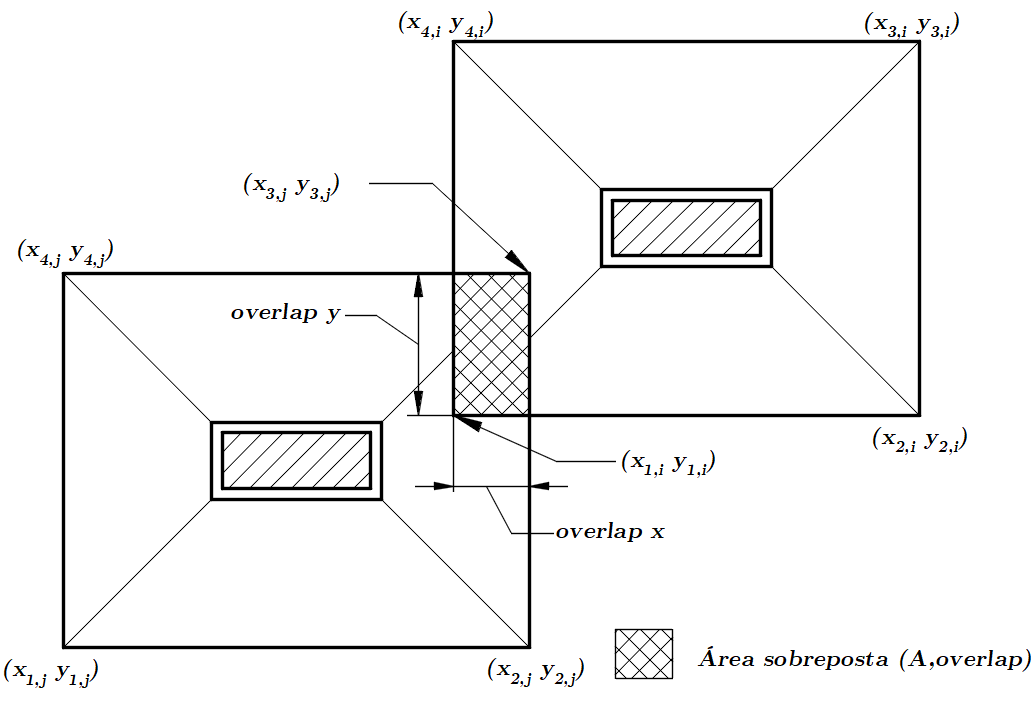
\includegraphics[width=0.9\linewidth]{figuras/sobreposição.png}
    \caption{Área de sobreposição entre duas sapatas.}
    \label{fig:sobreposição}
\end{figure}

Cada sapata é definida pelas coordenadas de seus vértices através das Equações \eqref{eq:coord_x1} a \eqref{eq:coord_y4}.
\begin{equation}
x_{1,i} = x_{g,i} - \frac{h_{x,i}}{2},
\label{eq:coord_x1}
\end{equation}

\begin{equation}
y_{1,i} = y_{g,i} - \frac{h_{y,i}}{2},
\label{eq:coord_y1}
\end{equation}

\begin{equation}
x_{2,i} = x_{g,i} + \frac{h_{x,i}}{2},
\label{eq:coord_x2}
\end{equation}

\begin{equation}
y_{2,i} = y_{g,i} - \frac{h_{y,i}}{2},
\label{eq:coord_y2}
\end{equation}

\begin{equation}
x_{3,i} = x_{g,i} + \frac{h_{x,i}}{2},
\label{eq:coord_x3}
\end{equation}

\begin{equation}
y_{3,i} = y_{g,i} + \frac{h_{y,i}}{2},
\label{eq:coord_y3}
\end{equation}

\begin{equation}
x_{4,i} = x_{g,i} - \frac{h_{x,i}}{2},
\label{eq:coord_x4}
\end{equation}

\begin{equation}
y_{4,i} = y_{g,i} + \frac{h_{y,i}}{2}.
\label{eq:coord_y4}
\end{equation}

A partir da análise simultânea de dois elementos de sapatas, chamadas de $i$ e $j$, é possível identificar o comprimento de sobreposição, denominado $overlap$, para as direções $x$ e $y$, obtidos através das Equações \eqref{eq:overlap_x} e \eqref{eq:overlap_y}.

\begin{equation}
\text{overlap}_x = \max\left(0,\ \min(x_{i,\max},\, x_{j,\max}) - \max(x_{i,\min},\, x_{j,\min})\right),
\label{eq:overlap_x}
\end{equation}

\begin{equation}
\text{overlap}_y = \max\left(0,\ \min(y_{i,\max},\, y_{j,\max}) - \max(y_{i,\min},\, y_{j,\min})\right).
\label{eq:overlap_y}
\end{equation}

A área de sobreposição é obtida pelo produto dos comprimentos $overlap$, apresentado na Equação \eqref{eq:area_sobreposição}. Esse valor é utilizado na penalização de sobreposição.

\begin{equation}
    A_{overlap} = overlap_x \cdot overlap_y.
    \label{eq:area_sobreposição}
\end{equation}

\subsection{Punção}

A verificação da punção será realizada conforme prescrito pela NBR 6118 para elementos estruturais de concreto armado \cite{nbr6118}. Esse procedimento consiste na análise da resistência ao cisalhamento em superfícies críticas sucessivas, definidas no entorno da região de aplicação do carregamento do pilar.

O esforço de punção atua em dois perímetros críticos, designados por $C$ e $C'$, conforme ilustrado na Figura \ref{fig: perímetro_critico}. O perímetro $C$ corresponde ao contorno do pilar enquanto $C'$ indica a região crítica localizada a uma distância de $2d$ da borda do pilar, sendo $d$ a altura útil da sapata.

\begin{figure}[htbp!]
    \centering
    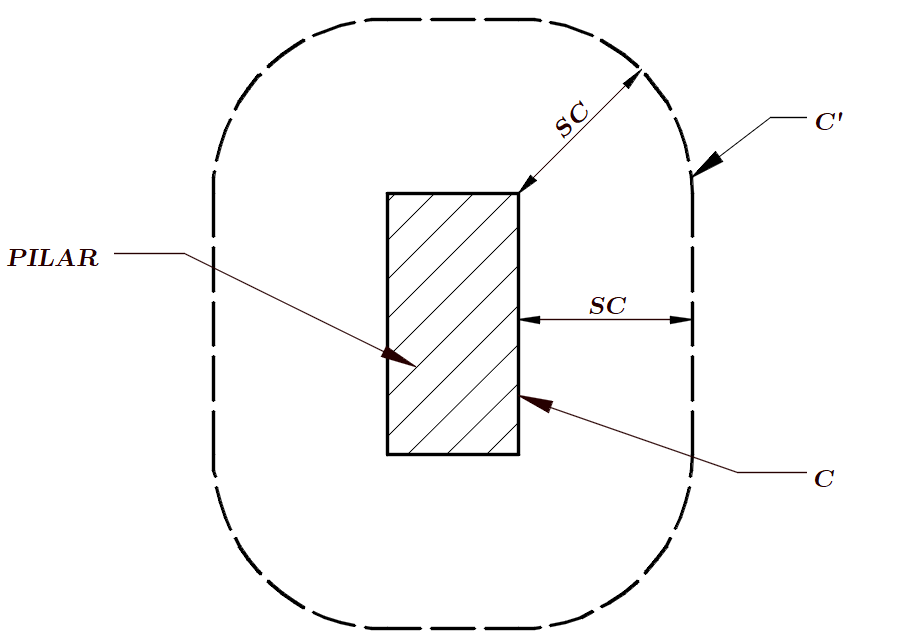
\includegraphics[width=0.5\linewidth]{figuras/perímetro_crítico.png}
    \caption{Perímetro crítico}
    \label{fig: perímetro_critico}
\end{figure}

A resistência da seção $C$ é determinada pela Equação~\eqref{eq:Tensão_resistente_C}

\begin{equation}
 \tau_{rd2} = 0,27 \cdot f_{cd} \cdot \alpha_{v2},
     \label{eq:Tensão_resistente_C}
\end{equation}

em que $f_{cd}$, a resistência de cálculo do concreto, é dado pela Equação \eqref{eq:fcd}

\begin{equation}
    f_{cd} = \frac{f_{ck}}{1,40},
        \label{eq:fcd}
\end{equation}

$\alpha_{v2}$ é definido pela Equação \eqref{eq:alpha_v2}, utilizando o valor de $f_{ck}$ em $MPa$

\begin{equation}
    \alpha_{v2} =  1 - \frac{f_{ck}}{250}.
        \label{eq:alpha_v2}
\end{equation}

 O cálculo da tensão solicitante de cálculo é dada pela Equação~\eqref{eq:Tensão_solicitante_C}.

\begin{equation}
 \tau_{sd2} = \frac{F_{zk} \cdot 1.4}{2 \cdot (a_p + b_p) \cdot d},
     \label{eq:Tensão_solicitante_C}
\end{equation}


em que $d$ é a altura útil, obtida pela Equação \eqref{eq:altura_util}, onde $cob$ indica o cobrimento mínimo da armadura.

\begin{equation}
    d = h_z - cob.
    \label{eq:altura_util}
\end{equation}


% O esforço de punção atua em dois perímetros críticos, designados por $C$ e $C'$, conforme ilustrado na figura. O perímetro $C$ corresponde ao contorno do pilar enquanto $C'$ indica a região crítica localizada a uma distância de $2d$ da borda do pilar, sendo $d$ a altura útil da sapata. Contudo a distância do perímetro $c'$, denominada na imagem como $SC$, será adotada a partir da expressão comumente utilizada de metade do $h_z$. 


% A verificação de punção consiste em definir a tensão solicitante ($\tau_{sd}$) e resistente ($\tau_{rd}$) para os dois perímetros. Assim sendo, para o perímetro $C$ tem-se os cálculos seguintes: Primeiramente, é definida a altura útil, Equação \eqref{eq:altura_util}. Em seguida, é determinada a tensão solicitante  no perímetro $C$ $\tau_{sd2}$ pela 


% Sendo $a_p$ e $b_p$ as dimensões do pilar em metros, nas direções de $x$ e $y$, respectivamente. $h_z$ é a altura do elemento de fundação em metros e $cob$ a espessura do cobrimento da armadura em metros. $f_{ck}$ e $f_{cd}$ são, respectivamente, a resistência característica e de cálculo do concreto em $MPa$.
% Em seguida, deve-se calcular a tensão resistente  no perímetro $C$ $\tau_{rd2}$, dada pela Equação \eqref{eq:Tensão_resistente_C}:



% No perímetro $C'$, a tensão resistente $\tau_{rd2}$ é dada pela Equação \eqref{eq:Tensão_resistente_C'}:

% \begin{equation}
%  \tau_{rd1} = 0,13 \cdot k_e \cdot \left( 100 \cdot \rho \cdot f_{ck} \right) ^\frac{1}{3}  + 0,1 \cdot \sigma_{cp}
%      \label{eq:Tensão_resistente_C'}
% \end{equation}

% Onde $k_e$ é o coeficiente de escala de punção identificado pela Equação \eqref{eq:ke}, $\rho$ é a taxa geométrica de armadura de flexão aderente, definida pela tabela ?????. $\sigma_{sp}$ é a tensão devida a ação de elementos protendidos.

% \begin{equation}
% k_e = 1 + \sqrt{\frac{20}{d \cdot 100}}
% \label{eq:ke}
% \end{equation}

% A tensão solicitante no perímetro $C'$ é dada pela \eqref{eq:Tensão_solicitante_C'}:

% \begin{equation}
%  \tau_{sd1} = \frac{1,4 \cdot F_{zk}}{u \cdot d} + \frac{1,4 \cdot k_x \cdot M_{xk}}{w_{px} \cdot d} + \frac{1,4 \cdot k_y \cdot M_{yk}}{w_{py} \cdot d}
%      \label{eq:Tensão_solicitante_C'}
% \end{equation}

% Nesta equação, $k_x$ e $k_y$ referem-se a coeficientes que indicam a parcela de transmissão do momento ao pilar por cisalhamento. Estes são obtidos pela tabela 19.2 da NBR 6118. $w_{px}$ e $w_{py}$ são definidos pelas Equações \eqref{eq:wpx} e \eqref{eq:wpy}, respectivamente. $d$ é a altura útil definida anteriormente neste item. $u$ representa o perímetro crítico $C'$ dado pela Equação \eqref{eq:perímetro_c'}.

% \begin{equation}
% w_{px} = \frac{a_p^2}{2} + a_p \cdot b_p + 4 \cdot b_p \cdot sc + 16 \cdot sc^2 + 2 \cdot \pi \cdot a_p \cdot sc
% \label{eq:wpx}
% \end{equation}

% \begin{equation}
% w_{py} = \frac{b_p^2}{2} + b_p \cdot a_p + 4 \cdot a_p \cdot sc + 16 \cdot sc^2 + 2 \cdot \pi \cdot b_p \cdot sc
%     \label{eq:wpy}
% \end{equation}

% \begin{equation}
% u = 2 \cdot \left( a_p + b_p \right) + 4 \pi \cdot sc 
%     \label{eq:perímetro_c'}
% \end{equation}


% Em que $sc$ representa a distância da seção crítica da borda do pilar conforme a figura \eqref{fig: perímetro_critico}, dada pela Equação \eqref{eq:secao_critica}:
% %\begin{equation}
% %u_{rd2} = 2 \cdot (a_p + b_p)
%  %   \label{eq:urd2}
% %\end{equation}


% \begin{equation}
% sc = \frac{h_z}{2}
%     \label{eq:secao_critica}
% \end{equation}


% Após definidas as tensões solicitantes e resistentes, são feitas as verificações aprepresentadas no item 4 deste trabalho.

% As equações a seguir talvez devam ir para a metodologia, pois são utilizadas pelo código para "interpretar" tabelas da norma:

% \begin{equation}
% rho = \frac{\sqrt{rho_x * rho_y}}{100}
%     \label{eq:rho}
% \end{equation}

% \begin{equation}
% C1\_C2 = \frac{a_p}{b_p}
%     \label{eq:c1-C2}
% \end{equation}

% \begin{equation}
% C2\_C1 = \frac{b_p}{a_p}
%     \label{eq:C2-C1}
% \end{equation}

\section{Otimização baseada em aprendizado de máquina}\label{sec:ego}A otimização híbrida surge como uma abordagem eficaz para lidar com problemas de otimização global caracterizados por funções objetivo de elevado custo computacional. Nesses cenários, a aplicação direta de métodos clássicos de otimização torna-se impraticável, motivando o desenvolvimento de estratégias que reduzam o número de avaliações reais da função \cite{Jones1998,Forrester2008}.

O princípio fundamental da otimização híbrida consiste na combinação de modelos aproximados (\textit{surrogates}) com estratégias de busca global. Em particular, a maior parte das avaliações diretas da função objetivo é substituída por predições fornecidas por um modelo de baixo custo computacional, enquanto avaliações reais são realizadas de forma seletiva e orientada. Essa estratégia permite reduzir significativamente o custo computacional total do processo de otimização, sem comprometer a capacidade de exploração global do espaço de busca \cite{Jones1998}.

Neste trabalho, adota-se uma estratégia híbrida de otimização baseada em aprendizado de máquina, fundamentada no método \textit{Efficient Global Optimization} (EGO). Esta abordagem será combinada com um algoritmo genético para assegurar a convergência a um ótimo global da função mono-objetivo.

\subsection{Problema mono-objetivo}

Um problema de otimização mono-objetivo ($SOO - Single \; Objective \;Optimization$) busca um resultado ótimo em um ponto do espaço de projeto que minimiza (ou maximiza) apenas uma função objetivo \cite{moreira}. Semelhante aos problemas multiobjetivos, a formulação de um problema mono-objetivo inclui um conjunto de restrições. Essas restrições representam condições que qualquer solução considerada viável deve obrigatoriamente satisfazer. Desse modo, a busca pela solução ótima ocorre apenas dentro do espaço de soluções que atendam às restrições estabelecidas. O conjunto de equações representado em \eqref{eq:problema_otimizacao} apresenta a forma genérica de um problema mono-objetivo:

\begin{equation}
\left\{\; \;
\begin{aligned}
& \min f(\textbf{X}), \\[0.3em]
& g_i(\textbf{X}) \le 0, \quad i = 1, 2, \dots, J, \\[0.3em]
& h_j(\textbf{X}) = 0, \quad j = 1, 2, \dots, K, \\[0.3em]
& x_i^L \le x_i \le x_i^U, \quad i = 1, 2, \dots, n.
\end{aligned}
\right.
\label{eq:problema_otimizacao}
\end{equation}
\vspace{1em}

A formulação envolve uma função objetivo $f(\textbf{X})$, onde X representa o vetor das variáveis de projeto. As inequações $g_j (\textbf{X})$, as equações $h_k (\textbf{X})$ e os limites laterais $x_i^L$ e $x_i^U$ correspondem às restrições que delimitam o espaço de busca viável. Os índices $j$, $k$ e $i$ identificam, respectivamente, as restrições de desigualdade, de igualdade e o intervalo de busca, enquanto $J$, $K$ e $n$ representam as quantidades totais desses elementos.

\subsection{Efficient Global Optimization (EGO)}
 
 Proposto por Jones, Schonlau e Welch \cite{Jones1998}, o EGO é um método de otimização global voltado para problemas em que a avaliação da função objetivo tem alto custo computacional. A ideia central do EGO é reduzir o número de avaliações diretas da função \textit{black-box} por meio de um modelo substituto (do inglês \textit{surrogate}), que aprende uma aproximação da função a partir de um conjunto inicial de amostras e é atualizado iterativamente ao longo do processo.

Em cada iteração, o EGO ajusta um modelo probabilístico (tipicamente um Processo Gaussiano/\textit{kriging}) e utiliza uma função de aquisição para decidir qual ponto deve ser avaliado a seguir. Essa função de aquisição quantifica um critério de utilidade que balanceia dois objetivos concorrentes: (i) explorar regiões do espaço de busca, onde a incerteza do modelo é alta (exploração) e (ii) intensificar a busca em regiões promissoras, onde a predição indica valores baixos da função objetivo (intensificação). Uma escolha clássica de função de aquisição no EGO é o \textit{Expected Improvement} (EI), que mede a melhoria esperada em relação ao melhor valor observado até o momento \cite{Jones1998,Shahriari2016}.

Na perspectiva de aprendizado de máquina, o EGO pode ser interpretado como uma arquitetura de aprendizado ativo. Diferentemente de abordagens passivas, nas quais o modelo é treinado sobre um conjunto fixo de dados, o EGO seleciona iterativamente novos pontos de amostragem com base em um critério de decisão que maximiza a expectativa de melhoria ou o ganho informacional. Essa interpretação se alinha à literatura de otimização Bayesiana e projeto sequencial de experimentos, na qual funções de aquisição são tratadas como utilidades para decidir novas avaliações com orçamento limitado \cite{Shahriari2016,SCHULZ20181, Snoek2012}.

Esse tipo de abordagem também aparece em aplicações recentes de projeto computacional: Deng Paulson e Messner (\cite{Deng2026_MetamaterialAL}) propõem um método \textit{gradient-free} para o projeto de metamateriais que usa a Regressão por Processo Gaussiano (GPR) para representar o campo de densidade, comprime a representação (matriz de covariância) para reduzir a dimensionalidade e, no espaço comprimido, emprega um método de \textit{active learning} (BADS — \textit{Bayesian Adaptive Direct Search}) para explorar o espaço de projeto de forma eficiente \cite{Deng2026_MetamaterialAL}.

\subsection{Regressão por Processo Gaussiano (GPR)}


No contexto do EGO, o modelo substituto é tipicamente formulado por meio de Regressão por Processo Gaussiano (GPR), também associada à tradição de \textit{kriging} na literatura de experimentos computacionais e superfícies de resposta \cite{Jones1998,Shahriari2016}. Diferentemente de modelos paramétricos, que assumem previamente uma forma funcional fixa, o GPR adota uma perspectiva Bayesiana não paramétrica, na qual se define uma distribuição de probabilidade sobre funções. Essa característica é particularmente adequada em problemas de otimização nos quais a função objetivo é desconhecida, cara de avaliar e pode apresentar comportamento não linear ou multimodal \cite{NIPS1995_7cce53cf,SCHULZ20181,Shahriari2016}.

Formalmente, assume-se que a função latente \(f(\mathbf{x})\) segue um processo gaussiano,
\begin{equation}
    f(\mathbf{x}) \sim \mathcal{GP}\!\big(m(\mathbf{x}),\,k(\mathbf{x},\mathbf{x}')\big),
\end{equation}
em que \(m(\mathbf{x})\) é a função média e \(k(\mathbf{x},\mathbf{x}')\) é a função de covariância, ou \textit{kernel}. No GPR, o \textit{kernel} desempenha papel central, pois é ele que define a estrutura de dependência entre os pontos do espaço de entrada. Em termos de modelagem, deseja-se especificar covariâncias de modo que pontos com entradas próximas produzam predições semelhantes \cite{NIPS1995_7cce53cf}. Assim, o \textit{kernel} codifica hipóteses iniciais sobre regularidade, suavidade e escala de variação da função, além de controlar como a informação observada em um ponto se propaga para regiões vizinhas do domínio \cite{NIPS1995_7cce53cf,SCHULZ20181}. Em problemas práticos, as observações podem ser descritas por
\begin{equation}
    y = f(\mathbf{x}) + \varepsilon,
\end{equation}
onde \(\varepsilon\) representa ruído observacional, usualmente modelado como gaussiano \cite{SCHULZ20181,Shahriari2016}.

Dado um conjunto de dados \(D=\{X,\mathbf{y}\}\), o GPR fornece, para qualquer ponto não observado \(\mathbf{x}\), uma distribuição preditiva gaussiana caracterizada por média \(\mu(\mathbf{x})\) e variância \(\sigma^2(\mathbf{x})\). Na forma clássica, a predição posterior pode ser escrita como
\begin{equation}
    \mu(\mathbf{x}) = K(\mathbf{x},X)\big(K(X,X)+\sigma_\varepsilon^2 I\big)^{-1}\mathbf{y},
\end{equation}
\begin{equation}
    \sigma^2(\mathbf{x}) = k(\mathbf{x},\mathbf{x}) - K(\mathbf{x},X)\big(K(X,X)+\sigma_\varepsilon^2 I\big)^{-1}K(X,\mathbf{x}),
\end{equation}
em que \(K(X,X)\) é a matriz de covariância entre os pontos amostrados \cite{NIPS1995_7cce53cf}. A média preditiva expressa a melhor estimativa do valor da função, enquanto a variância quantifica a incerteza associada ao modelo em cada região do domínio. Como ambas dependem diretamente da função de covariância, a escolha do \textit{kernel} afeta simultaneamente a qualidade da aproximação e a forma como a incerteza é distribuída no espaço de busca \cite{NIPS1995_7cce53cf}.

Essa quantificação explícita de incerteza é precisamente o que torna o GPR particularmente apropriado para o EGO. Como a otimização Bayesiana é um procedimento sequencial baseado em modelo probabilístico, o \textit{surrogate} precisa não apenas aproximar a função objetivo, mas também indicar onde essa aproximação é menos confiável \cite{Shahriari2016}. Nesse sentido, \(\mu(\mathbf{x})\) sustenta a intensificação em regiões promissoras, ao passo que \(\sigma(\mathbf{x})\) viabiliza a exploração de regiões ainda pouco conhecidas. No EGO, essa dualidade é explorada por funções de aquisição como o \textit{Expected Improvement}, que utilizam simultaneamente predição e incerteza para decidir a próxima avaliação cara da função \cite{Jones1998,Shahriari2016}.

Além disso, o desempenho do GPR depende da escolha do \textit{kernel} e de seus hiperparâmetros. Em Williams e Rasmussen, por exemplo, os parâmetros da covariância controlam a escala das correlações locais, a contribuição de componentes lineares e de viés, bem como a variância do ruído; em particular, diferentes pesos por dimensão permitem refletir a relevância relativa de cada variável de entrada \cite{NIPS1995_7cce53cf}. Assim, no EGO, o GPR atua como um \textit{surrogate} probabilístico capaz de combinar flexibilidade funcional, interpolação não linear e quantificação de incerteza, reduzindo o número de avaliações reais necessárias em problemas de otimização de alto custo computacional \cite{Jones1998,Shahriari2016}.
\subsection{Critério de aquisição: \textit{Expected Improvement} (EI)}

Considere um conjunto de amostras $X=\{\mathbf{x}_1,\ldots,\mathbf{x}_n\}$ e respostas $Y=\{y_1,\ldots,y_n\}$, obtidas ao avaliar a função cara $F(\cdot)$ a ser minimizada. Denote o melhor valor observado por:

\begin{equation}
f_{\min}=\min\{y_1,y_2,\ldots,y_n\}.
\end{equation}

Assumindo que o \textit{surrogate} fornece, para cada $\mathbf{x}$, uma distribuição preditiva normal

\begin{equation}
Y(\mathbf{x}) \sim \mathcal{N}\big(\mu(\mathbf{x}),\,\sigma^2(\mathbf{x})\big),
\end{equation}

em que $Y(\mathbf{x})$ é a variável aleatória que modela o valor da função objetivo real. $\mathcal{N}$ Indica que a distribuição é normal (gaussiana), $\mu(\mathbf{x})$ representa a melhor estimativa do modelo para o valor da função objetivo. $\sigma^2(\mathbf{x})$ é a variância da distribuição preditiva. Sua raiz quadrada, 
$\sigma(\mathbf{x})$, é o desvio padrão, que quantifica a incerteza do modelo. Em seguida define-se a melhoria aleatória

\begin{equation}
I(\mathbf{x})=\max\big(f_{\min}-Y(\mathbf{x}),\,0\big),
\end{equation}

e a função de aquisição como sua esperança:

\begin{equation}
\mathrm{EI}(\mathbf{x})=\mathbb{E}[I(\mathbf{x})].
\end{equation}

No caso gaussiano, obtém-se uma forma fechada \cite{Jones1998} para a função de aquisição:

\begin{equation}
\mathrm{EI}(\mathbf{x})=
\big(f_{\min}-\mu(\mathbf{x})\big)\,
\Phi\!\left(\frac{f_{\min}-\mu(\mathbf{x})}{\sigma(\mathbf{x})}\right)
+\sigma(\mathbf{x})\,
\phi\!\left(\frac{f_{\min}-\mu(\mathbf{x})}{\sigma(\mathbf{x})}\right),
\label{eq:ei_closed_form}
\end{equation}

onde $\Phi(\cdot)$ e $\phi(\cdot)$ são, respectivamente, a CDF (\textit{Cumulative Distribution Function}) e a PDF (\textit{Probability Density Function}) da normal padrão. A Equação~\eqref{eq:ei_closed_form} é o ponto-chave: o termo com $\Phi(\cdot)$ favorece intensificação quando a média predita melhora $f_{\min}$, enquanto o termo com $\phi(\cdot)$ cresce com $\sigma(\mathbf{x})$, favorecendo exploração em regiões incertas \cite{Jones1998,Shahriari2016}.

\subsection{Otimizador interno}\label{sec:otm_interno}

Uma vez construído o modelo substituto (\textit{surrogate} model), a maximização do \textit{Expected Improvement} (EI) que é expresso pela Equação~\eqref{eq:ei_closed_form} é conduzida por um otimizador interno baseado em metaheurística. Neste trabalho, adotou-se um Algoritmo Genético (AG), implementado por meio da biblioteca \textsc{MEALPY} \cite{van2023mealpy, van2023groundwater}, cujos fundamentos e parametrização são descritos a seguir.

O Algoritmo Genético é uma metaheurística inspirada nos mecanismos da evolução natural e na seleção darwiniana \cite{holland1992}. Seu funcionamento básico consiste em evoluir iterativamente uma população de soluções candidatas (indivíduos) por meio dos operadores de \textbf{seleção}, \textbf{cruzamento} e \textbf{mutação}, preservando as características mais promissoras ao longo das gerações. Um fluxograma esquemático do processo é apresentado na Figura~\ref{fig:fluxograma_AG}.

\begin{figure}[H]
  \centering
  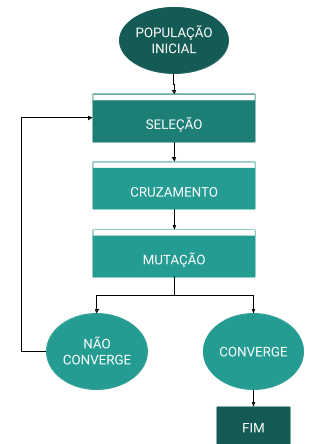
\includegraphics[width=0.4\textwidth]{figuras/fluxograma_AG.png}
  \caption{Fluxograma representativo do Algoritmo Genético.}
  \label{fig:fluxograma_AG}
\end{figure}

O AG inicia com uma população aleatória de indivíduos, cada um representando um ponto no espaço de busca. A cada geração, os indivíduos são avaliados segundo uma função de aptidão. Os mais aptos têm maior probabilidade de serem selecionados para reprodução, gerando novos indivíduos que gradualmente convergem para regiões de maior interesse.

\subsubsection{Operadores genéticos adotados}

\textbf{Seleção por roleta}: Utilizou-se o método da roleta (\textit{roulette wheel selection}), no qual cada indivíduo recebe uma probabilidade de seleção proporcional à sua aptidão relativa. Isso permite que indivíduos menos aptos ainda possam ser escolhidos, mantendo a diversidade populacional e reduzindo o risco de convergência prematura \cite{linden}.

\textbf{Cruzamento linear}: Dois indivíduos selecionados \( p_0 \) e \( p_1 \) são combinados para gerar três descendentes por combinação linear de suas variáveis de projeto:

\begin{equation}
\begin{aligned}
{des}_{a,k} &= 0{,}50 \cdot p_{0,k}^{t} + 0{,}50 \cdot p_{1,k}^{t},\\[2pt]
{des}_{b,k} &= 1{,}50 \cdot p_{0,k}^{t} - 0{,}50 \cdot p_{1,k}^{t},\\[2pt]
{des}_{c,k} &= -0{,}50 \cdot p_{0,k}^{t} + 1{,}50 \cdot p_{1,k}^{t},
\end{aligned}
\label{eq:desc_crossover}
\end{equation}

onde \( k \) indica a \( k \)-ésima variável e \( t \) a geração atual. O melhor descendente é então selecionado para compor a nova população:

\begin{equation}
\mathbf{x}^{(t+1)} = \arg\min\bigl\{ {des}_{a,k},\, {des}_{b,k},\, {des}_{c,k} \bigr\}.
\label{eq:melhor_des}
\end{equation}

\textbf{Mutação por \textit{hill‑climbing} com perturbação gaussiana}: Para explorar regiões vizinhas à solução atual, aplica‑se um operador de mutação baseado em uma perturbação gaussiana:
\begin{equation}
x_{i,k}^{(t+1)} \sim \mathcal{N}\!\left(x_{i,k}^{t},\, \sigma\right),
\qquad
\sigma = x_{i,k}^{t} \cdot \frac{\mathit{cov}}{100},
\label{eq:mutacao_gaussiana}
\end{equation}
em que \( \mathcal{N}(\mu,\sigma) \) denota uma distribuição normal com média \( \mu \) e desvio padrão \( \sigma \), e \( \mathit{cov} \) é um coeficiente de variação definido pelo usuário. Este mecanismo introduz diversidade sem abandonar completamente a informação já acumulada.

\subsection{Fluxo operacional do EGO}

O EGO executa um ciclo iterativo modelar $\rightarrow$ selecionar $\rightarrow$ avaliar $\rightarrow$ atualizar, como apresentado na Figura \ref{fig:Fluxograma_EGO}.

\begin{figure}[H]
    \centering
    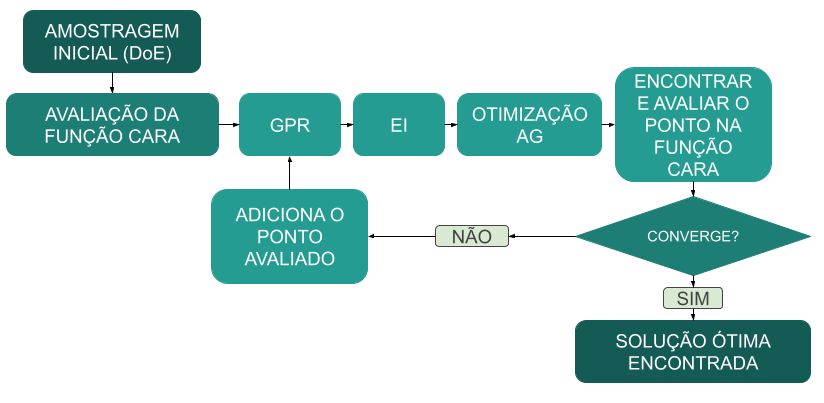
\includegraphics[width=0.7\linewidth]{figuras/fluxograma_EGO.png}
    \caption{Fluxograma operacional do EGO.}
    \label{fig:Fluxograma_EGO}
\end{figure}

Em forma objetiva, tem-se:
\begin{enumerate}
    \item \textbf{Projeto de Experimentos (DoE -- \textit{Design of Experiments}) inicial:} escolher um conjunto inicial $X$ com boa cobertura do domínio (por exemplo, \textit{Latin Hypercube}) e avaliar $Y$ \cite{Jones1998}.
    \item \textbf{Treinamento do \textit{surrogate}:} ajustar o modelo probabilístico aos dados $(X,Y)$ para obter $\mu(\mathbf{x})$ e $\sigma(\mathbf{x})$ (ou $\sigma^2(\mathbf{x})$) \cite{Jones1998}.
    \item \textbf{Construção da aquisição:} calcular $\mathrm{EI}(\mathbf{x})$.
    \item \textbf{Escolha do próximo ponto:} resolver
    \begin{equation}
        \mathbf{x}_{n+1}=\arg\max_{\mathbf{x}\in\mathcal{X}} \mathrm{EI}(\mathbf{x}),
    \end{equation}

    em que o termo $\arg\max$ retorna o ponto que maximiza a função. Em seguida avalia $y_{n+1}=F(\mathbf{x}_{n+1})$
    \item \textbf{Atualização:} incorporar $(\mathbf{x}_{n+1},y_{n+1})$ ao conjunto e repetir a partir do passo 2 \cite{Jones1998}.
\end{enumerate}

A iteração prossegue até um orçamento máximo de avaliações ou até que o ganho esperado se torne marginal (por exemplo, $\max_{\mathbf{x}}\mathrm{EI}(\mathbf{x})$ suficientemente pequeno), indicando baixo retorno incremental para novas amostras \cite{Jones1998,Shahriari2016}.






\section{Metodologia}\label{sec:method}O dimensionamento otimizado de sapatas é formulado como um problema de 
otimização com restrições, cujo objetivo é determinar as dimensões 
geométricas que atendam simultaneamente aos requisitos normativos e de 
viabilidade construtiva, minimizando o volume total de concreto.

As restrições são expressas como \( g_j(\mathbf{X}) \le 0 \), em que 
valores positivos de \( g_j \) representam violações. Para incorporá-las 
a um esquema de otimização irrestrita, adota-se uma função de penalização 
quadrática, definida por:

\begin{equation}
P(\mathbf{X}) = \alpha \sum_{j=1}^{N} \max\bigl(0, g_j(\mathbf{X})\bigr)^2,
\label{eq:penalizacao}
\end{equation}

onde \( N \) é o número de restrições e \( \alpha \) é um coeficiente de 
penalidade, garantindo que soluções inviáveis sejam 
severamente desfavorecidas.

A função objetivo final \( \Theta(\mathbf{X}) \) é então composta pelo 
somatório dos volumes das sapatas, acrescido do termo de penalização:

\begin{equation}
\Theta(\mathbf{X}) = V_{\text{total}}(\mathbf{X}) + P(\mathbf{X}).
\label{eq:funcao_pseudo_objetivo}
\end{equation}

Dessa forma, o problema original com restrições é transformado em um 
problema irrestrito de minimização de uma \textit{função pseudo-objetivo} 
\( \Theta(\mathbf{X}) \), onde soluções factíveis (\( P = 0 \)) correspondem 
estritamente à minimização do volume estrutural.

\subsection{Restrições de tensões no solo}


As restrições associadas as tensões de contato entre a sapata e o solo são formuladas de modo a garantir que as tensões solicitantes máximas e mínimas permaneçam dentro dos limites admissíveis do solo e assim, assegurem que não ocorram tensões maiores que a capacidade do solo, nem tensões de tração no contato entre o solo e a sapata.

A restrição associada à tensão máxima é expressa pela Equação\eqref{eq:restricao_tensão_máx}:

\begin{equation}
g_{tensao}^{max} = \frac{\sigma_{sd}}{\sigma_{adm}} - 1.
    \label{eq:restricao_tensão_máx}
\end{equation}

Da mesma forma, a restrição associada à tensão mínima é dada pela Equação \eqref{eq:restricao_tensão_min}. Salienta-se aqui que essa restrição é dada neste formato visto que não será admitida tração neste trabalho.

\begin{equation}
g_{tensao}^{min} = \frac{-\sigma_{sd}}{\sigma_{adm}}.
    \label{eq:restricao_tensão_min}
\end{equation}

\subsection{Restrição geometria pilar-sapata}

A compatibilidade geométrica em planta é garantida assegurando que as dimensões da sapata excedam as dimensões do pilar somadas à uma folga $\delta$ de cada lado do pilar. As Equações \eqref{eq:checagem_geometria_x} e \eqref{eq:checagem_geometria_y} estabelecem essas restrições para as direções $x$ e $y$, respectivamente.

\begin{equation}
g_{geometria,x} = 1 + \frac{2 \cdot \delta }{a_p} -  \frac{h_x}{a_p},
    \label{eq:checagem_geometria_x}
\end{equation}

\begin{equation}
g_{geometria,y} = 1 + \frac{2 \cdot \delta }{b_p} -  \frac{h_y}{b_p},
    \label{eq:checagem_geometria_y}
\end{equation}


em que $a_p$ e $b_b$ representam as dimensões do pilar, $h_x$ e $h_y$ representam as dimensões da sapata, enquanto o valor de $\delta$ indica a folga mínima entre o pilar e a lateral do elemento de fundação.

\subsection{Restrição de sobreposição}

A restrição de sobreposição tem como objetivo impedir que duas ou mais sapatas ocupem, simultaneamente, a mesma posição em planta, condição que inviabilizaria a execução da fundação.

Cada sapata é modelada geometricamente como um retângulo no plano, definido a partir das coordenadas de seus vértices, conforme descrito na Seção \ref{subsec:projeto_sobreposicao}. A partir da interseção geométrica entre dois retângulos, é possível definir a área de sobreposição ($A_{overlap}$) da sapata em análise. Esse valor é então aplicado na restrição definida pela Equação~\eqref{eq:restricao_sobreposicao}, na qual se obtém a razão entre a área de sobreposição da sapata analisada e sua área total em planta.

\begin{equation}
g_{sobreposicao} = \frac{A_{overlap}}{h_x \cdot h_y}.
    \label{eq:restricao_sobreposicao}
\end{equation}

\subsection{Restrição de punção}

A restrição associada à verificação da punção é formulada a partir da razão entre as tensão solicitante e a tensão admissível de cálculo correspondente, resultando em um valor adimensional ideal para o processo de otimização.

Para a seção crítica junto ao pilar (Seção $C$), define-se a Equação \eqref{eq:restricao_tensao_c}:
\begin{equation}
grd2 = \frac{\tau_{sd2}}{\tau_{rd2}}-1.
    \label{eq:restricao_tensao_c}
\end{equation}

\subsection{Configurações do algoritmo e métricas de acurácia}\label{sec:config_metricas}

A implementação do EGO desenvolvida nesta pesquisa permite flexibilidade na parametrização do processo Gaussiano e na escolha do otimizador interno. Enquanto os hiperparâmetros do Kriging foram calibrados conforme os resultados apresentados na Seção~\ref{sec:results}, o otimizador interno foi configurado com base em testes preliminares, os valores adotados constam na Tabela~\ref{tab:param_ag}.

\begin{table}[htpb!]
\centering
\caption{Parâmetros do Algoritmo Genético utilizado como otimizador interno.}
\begin{tabular}{@{}lc@{}}
\toprule
\textbf{Parâmetro} & \textbf{Valor} \\ 
\midrule
Tamanho da população ($pop\_size$) & 150 \\
Número de gerações ($epoch$) & 50 \\
Probabilidade de cruzamento ($pc$) & 0,95 \\
Probabilidade de mutação ($pm$) & 0,025 \\
\bottomrule
\end{tabular}
\label{tab:param_ag}
\end{table}

Embora a arquitetura desenvolvida admita a utilização de qualquer otimizador da biblioteca \textsc{SciPy} \cite{virtanen2020scipy} e \textsc{MEAPLY} \cite{van2023mealpy}, os resultados reportados neste trabalho restringem‑se ao AG, cujo desempenho foi validado preliminarmente. As demais possibilidades de otimizadores não foram exploradas sistematicamente e, portanto, não serão discutidas.

\subsubsection{Métricas de avaliação do modelo substituto}

Para quantificar a acurácia do modelo substituto (Kriging) em aproximar a função objetivo real, empregou‑se o coeficiente de determinação $R^2$, definido por:

\begin{equation}
R^2 = 1 - \frac{\displaystyle\sum_{i=1}^{n} \bigl( y_i - \hat{y}_i \bigr)^2}
                {\displaystyle\sum_{i=1}^{n} \bigl( y_i - \bar{y} \bigr)^2},
\label{eq:r2}
\end{equation}

onde $y_i$ é o valor real da função objetivo no ponto $i$, $\hat{y}_i$ é o valor predito pelo modelo, $\bar{y}$ é a média dos valores reais e $n$ é o número de pontos avaliados. Um valor de $R^2$ próximo a 1 indica que o modelo explica a maior parte da variabilidade dos dados.

% Para a seção crítica afastada do pilar (Seção $C'$) , tem-se a Equação \eqref{eq:grd1}:
% \begin{equation}
% g_{rd1} = \frac{\tau_{sd1}}{\tau_{rd1}} - 1
%     \label{eq:grd1}
% \end{equation}


% \subsection{balanço}
% O método exposto pelo CEB-70, indica um intervalo de balanço definido pela equação \eqref{eq:CEB-70 para direção x} e \eqref{eq:CEB-70 para direção y}.
% Modificando tais equações para adequá-lo ao formato de restrição utilizado o código tem-se as inequações \eqref{eq:restricao_balan_max_x} e \eqref{eq:restricao_balan_max_y} que indicam o limite máximo em $x$ e $y$, e as equações \eqref{eq:restricao_balan_min_x} e \eqref{eq:restricao_balan_min_y} que indicam o limite mínimo em $x$ e $y$, respectivamente. 
% \begin{equation}
% g_{0,balanço} = \frac{C_x}{2 \cdot h_z} - 1
%     \label{eq:restricao_balan_max_x}
% \end{equation}

% \begin{equation}
% g_{1,balanço} = \frac{C_y }{2 \cdot h_z} - 1
%     \label{eq:restricao_balan_max_y}
% \end{equation}

% \begin{equation}
% g_{2,balanço} = \frac{\frac{h_z }{2} }{C_x} - 1
%     \label{eq:restricao_balan_min_x}
% \end{equation}

% \begin{equation}
% g_{2,balanço} = \frac{\frac{h_z }{2} }{C_y} - 1
%     \label{eq:restricao_balan_min_y}
% \end{equation}
\section{Resultados}\label{sec:results}Esta seção apresenta os resultados do desenvolvimento da plataforma computacional e da aplicação do modelo de otimização EGO. A análise está organizada em três partes: (a) avaliação do desempenho do modelo substituto (\textit{Kriging}) e sua parametrização; (b) aplicação a um problema ilustrativo de dimensionamento de fundações, detalhando o fluxo de cálculo e a avaliação das restrições; e (c) descrição das funcionalidades da plataforma e da interação do usuário para obtenção de soluções otimizadas.

\subsection{Desempenho do modelo substituto}
\label{sec:desempenho_substituto}

Nesta seção, avalia-se o desempenho de um modelo substituto baseado em Regressão por Processos Gaussianos (GPR) para aproximar a função objetivo associada ao volume da fundações. A análise concentra-se em dois aspectos centrais: (\textit{i}) o impacto do fator de penalidade aplicado às restrições e (\textit{ii}) o efeito do aumento do número de amostras no conjunto de treinamento sobre a capacidade preditiva do modelo.

Diferentes funções de covariância (\textit{kernels}) foram avaliadas neste estudo, totalizando dezoito configurações distintas. Nesta seção, são apresentados os resultados referentes ao \textit{kernel} designado como \textbf{K06}, o qual consiste em uma variação parametrizada do \textit{kernel Matérn} 3/2.

Inicialmente, investigou-se a influência do fator de penalidade no comportamento da GPR. Para isso, considerou-se o \textit{kernel} \textbf{K06} e um particionamento fixo de dados ($70\%$ para treinamento e $30\%$ para teste), variando-se apenas o valor da penalidade aplicada às violações de restrição: uma penalidade suavizada ($\alpha=10^{1}$) e uma penalidade elevada ($\alpha=10^{6}$). A Figura~\ref{fig:impacto_penalidade} apresenta os gráficos de dispersão entre os valores observados e preditos para ambos os casos.

\begin{figure}[htpb!]
    \centering
    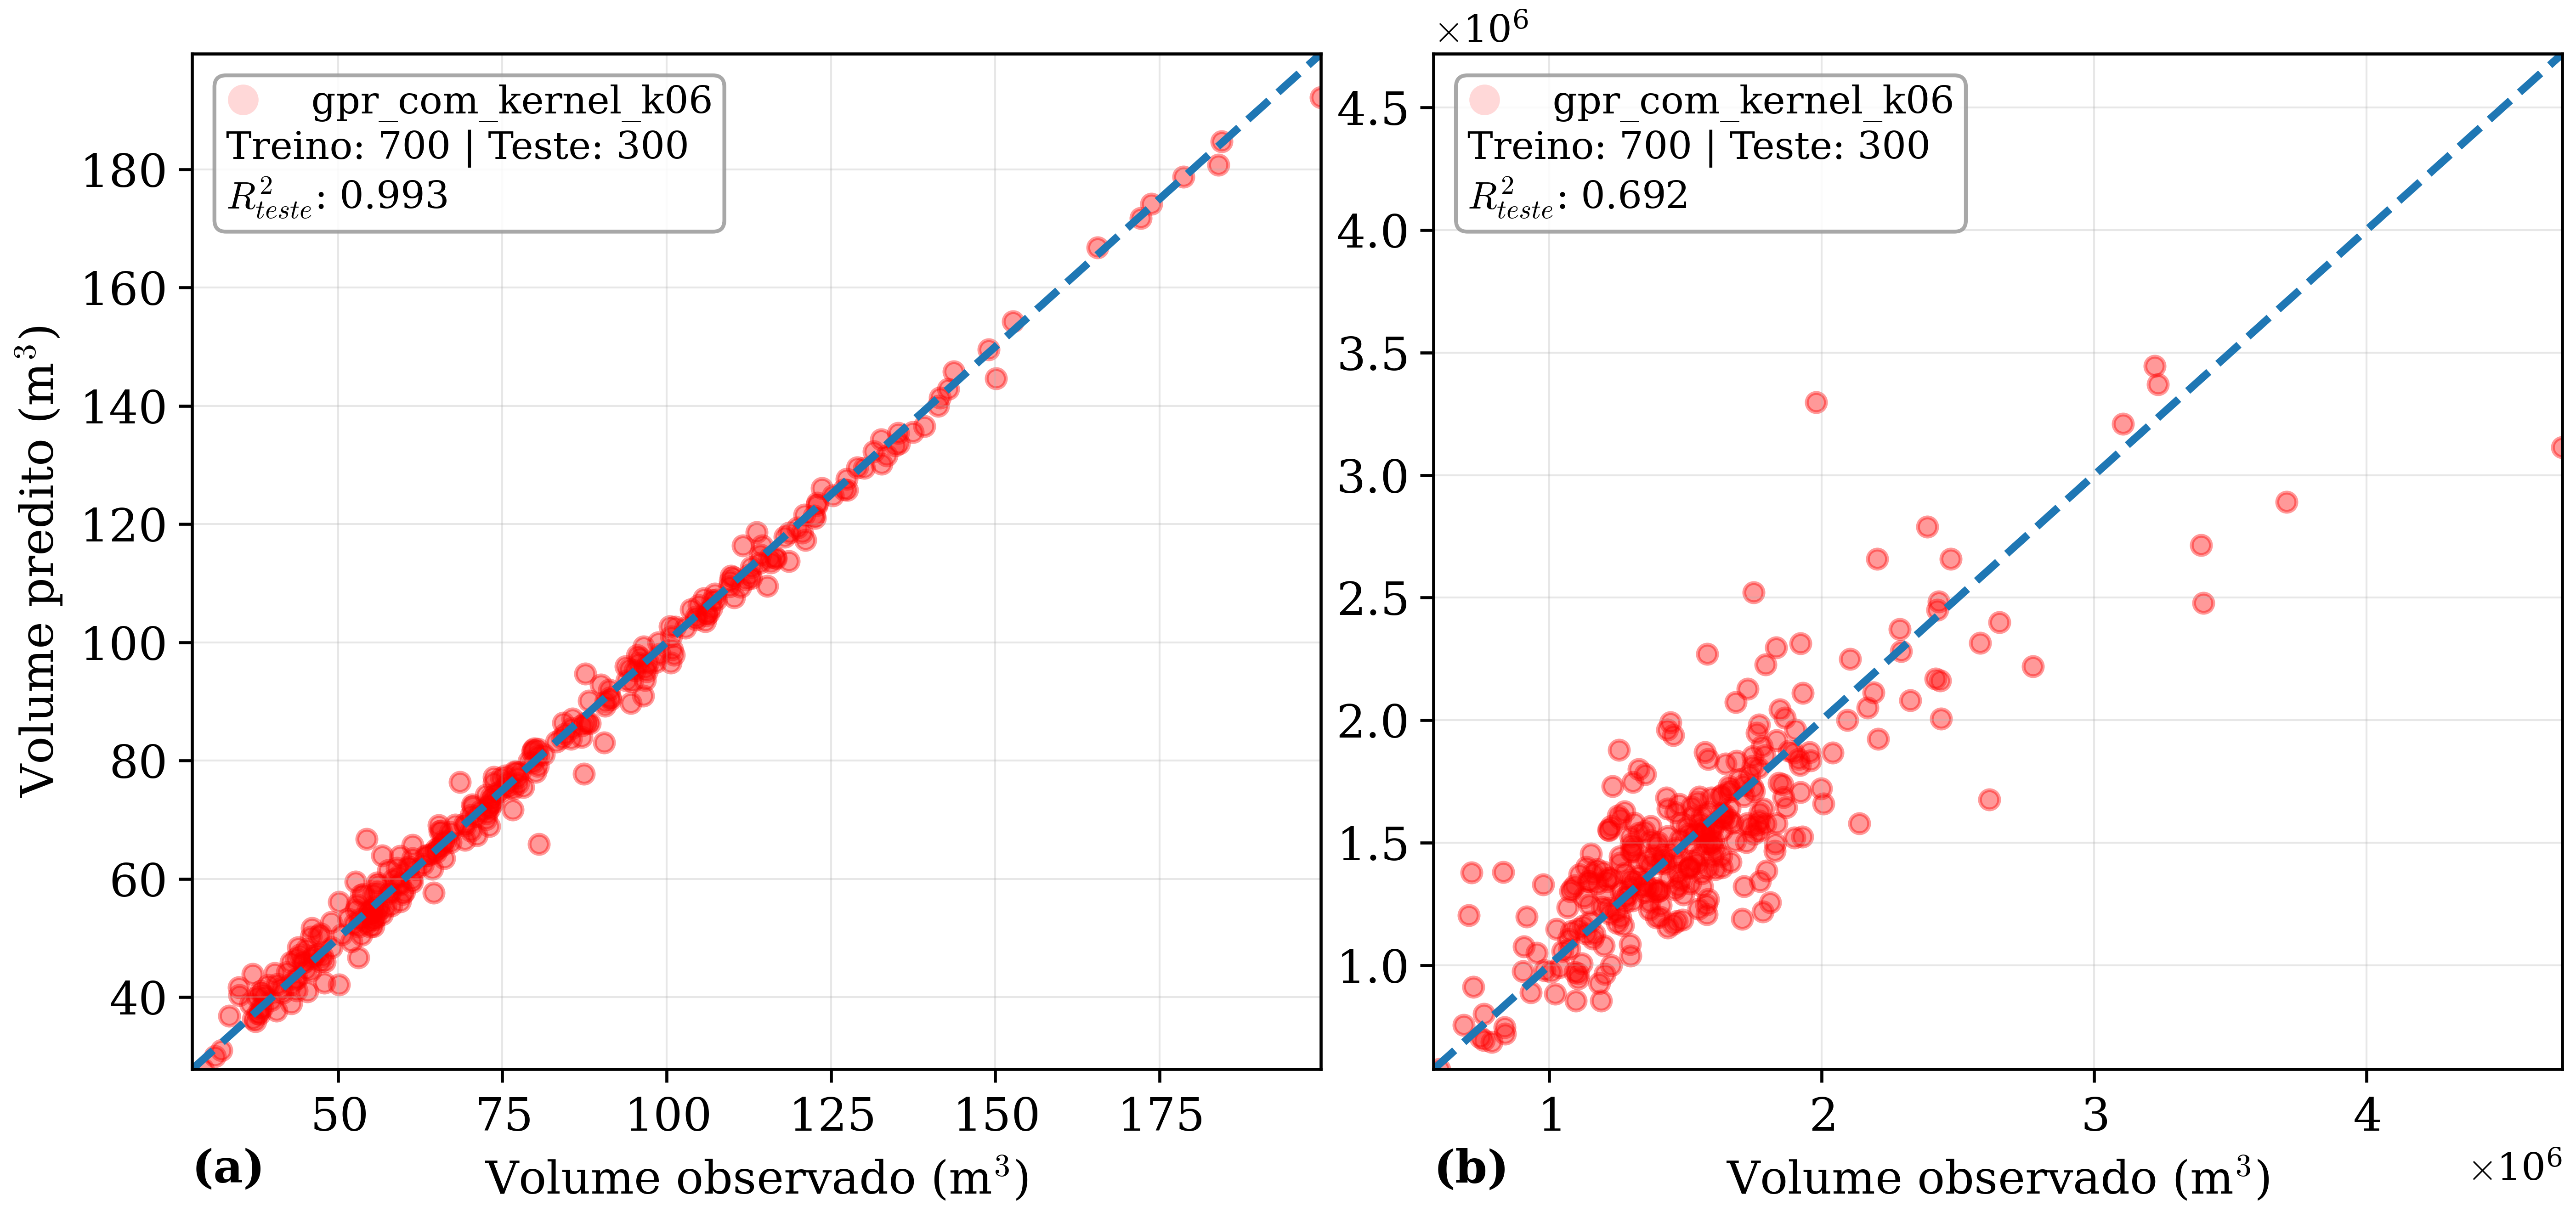
\includegraphics[width=\textwidth]{z_GPR_gpr_com_kernel_k06_pen_1e1_vs_1e6.png}
    \captionsetup{justification=centering}
    \caption{Gráficos de dispersão entre volumes observados e preditos pelo modelo GPR para o kernel k06, considerando (a) penalidade suavizada ($\alpha=10^{1}$) e (b) penalidade elevada ($\alpha=10^{6}$).}
    \label{fig:impacto_penalidade}
\end{figure}

Os resultados evidenciam que a adoção de penalidades elevadas induz uma mudança significativa na escala da função objetivo, com volumes penalizados atingindo ordens de grandeza da ordem de $10^{6}\,\mathrm{m}^3$. Essa amplificação compromete a capacidade do GPR de capturar a estrutura subjacente do problema, resultando em uma queda substancial no desempenho preditivo, com $R^2_{\mathrm{teste}} \approx 0{,}69$. Em contraste, a penalidade suavizada permite ao modelo representar adequadamente a relação entre as variáveis de decisão e o volume penalizado, alcançando valores elevados de coeficiente de determinação ($R^2_{\mathrm{teste}} \approx 0{,}99$). Esses resultados indicam que o fator de penalidade constitui um hiperparâmetro de grande importância em problemas de aprendizado ativo baseados em modelos substitutos.

Na sequência, foi avaliado o impacto do aumento do conjunto de treinamento no desempenho do GPR. Para essa análise, foram inicialmente testadas diferentes configurações de \textit{kernel} e, com base nas métricas no conjunto de teste, o \textit{kernel} \textbf{K06} foi escolhido como o mais promissor. A Figura~\ref{fig:impacto_treino} ilustra, para essa configuração (representativa do melhor desempenho), os gráficos de dispersão obtidos sob penalidade suavizada ($\alpha=10^{1}$) em dois cenários de particionamento: $90\%/10\%$ e $60\%/40\%$ (treino/teste).

\begin{figure}[htpb]
    \centering
    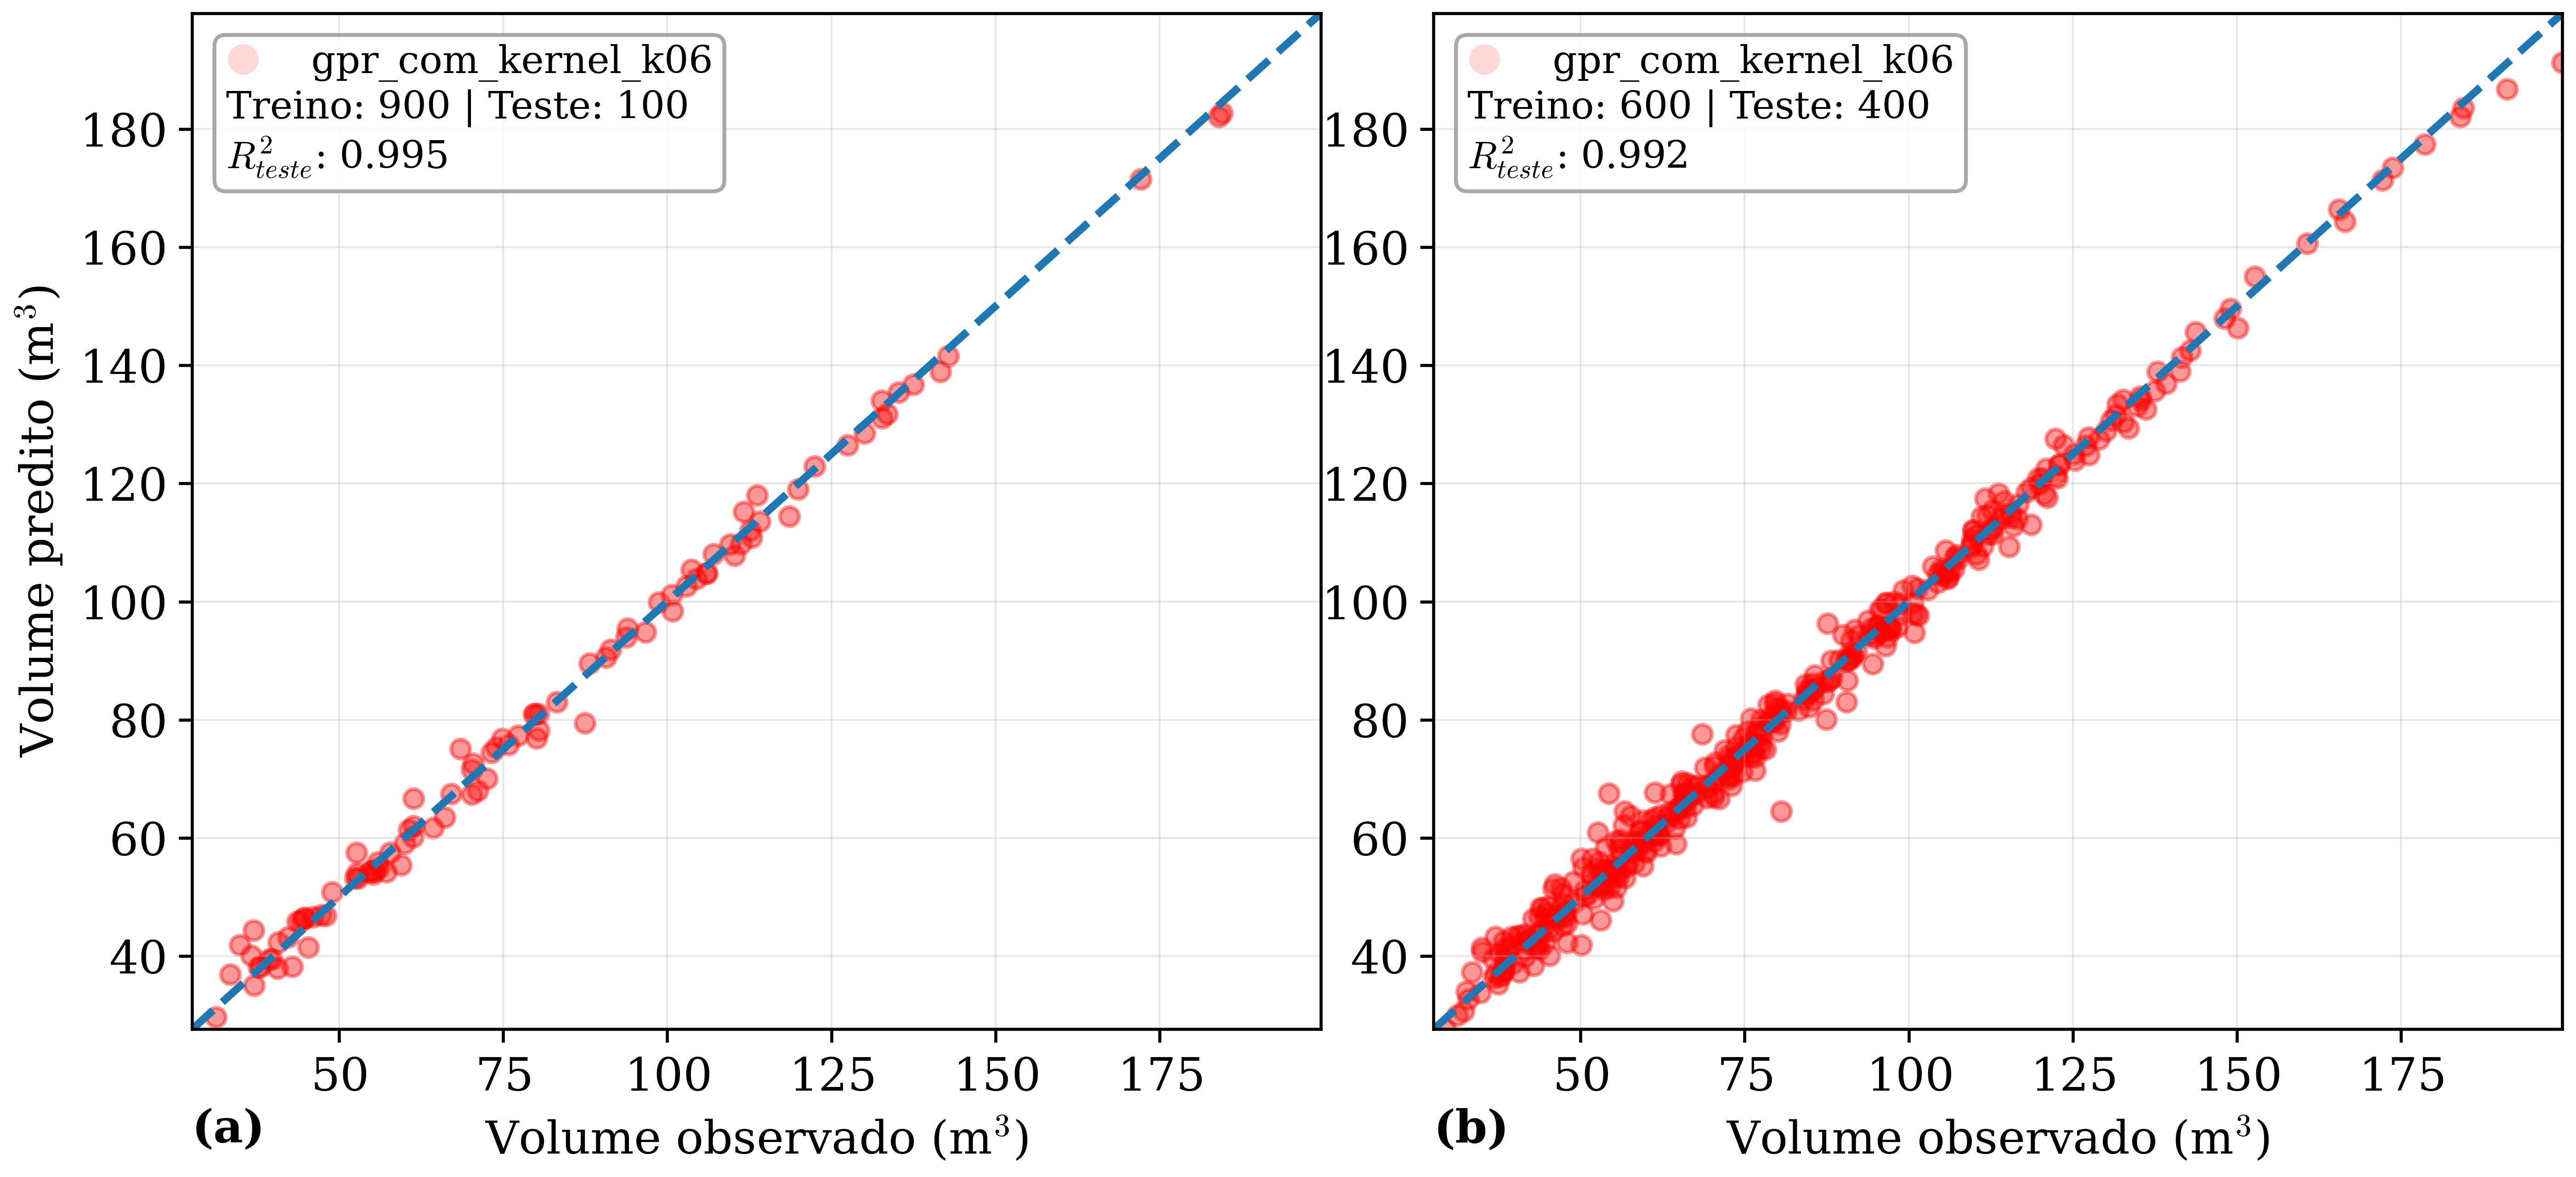
\includegraphics[width=\textwidth]{z_GPR_test_size_900_vs_600_comparison_gpr_com_kernel_k06.png}
    \captionsetup{justification=centering}
    \caption{Gráficos de dispersão entre volumes observados e preditos pelo modelo GPR para o kernel k06, considerando (a) $90\%/10\%$ (treino/teste) e (b) $60\%/40\%$ (treino/teste).}
    \label{fig:impacto_treino}
\end{figure}

Observa-se que o aumento do número de amostras de treinamento está associado a um incremento no coeficiente de determinação no conjunto de teste (de aproximadamente $0{,}992$ para $0{,}995$). Esse comportamento é consistente com o esperado em modelos estatísticos supervisionados: a ampliação do conjunto de treinamento tende a reduzir incertezas de estimação e a melhorar a aproximação da resposta, desde que as amostras sejam representativas do domínio de interesse.

Por fim, a Tabela~\ref{tab:metricas_gpr_toy_problem_all_splits} consolida as métricas de desempenho ($R^2_{\mathrm{test}}$, MAE e RMSE) para diferentes configurações de \textit{kernel}, considerando penalidade suavizada e múltiplos particionamentos treino/teste (\textit{test\_size} $\in \{0{,}10, 0{,}20, 0{,}30, 0{,}40, 0{,}50\}$). Essa análise justifica a escolha do \textit{kernel} adotado nas simulações subsequentes, destacando o desempenho superior do \textit{kernel} k06 no conjunto de teste. Ressalta-se que particionamentos com \textit{test\_size} reduzido (e.g., $0{,}10$) tendem a produzir estimativas de desempenho com maior variabilidade, uma vez que o conjunto de teste se torna menos representativo; por essa razão, a seleção do \textit{kernel} considerou a consistência das métricas ao longo dos diferentes particionamentos.

\begin{table}[H]
\centering
\caption{Métricas de desempenho dos modelos GPR para diferentes divisões treino/teste.}
\label{tab:metricas_gpr_toy_problem_all_splits}
\resizebox{\textwidth}{!}{%
\begin{tabular}{lcccccccccccccccccccc}
\toprule
\textbf{Kernel} & \textbf{Penalidade} & \textbf{Divisão} & \textbf{Treino} & \textbf{Teste} & $\mathbf{R^2_{\text{test}}}$ & \textbf{MAE}$\mathbf{_{\text{test}}}$ & \textbf{RMSE}$\mathbf{_{\text{test}}}$ \\
\midrule
gpr\_com\_kernel\_k06 & $10^{1}$ & 90/10 & 900 & 100 & 0.995 & 1.769 & 2.406 \\
gpr\_com\_kernel\_k18 & $10^{1}$ & 90/10 & 900 & 100 & 0.996 & 1.781 & 2.342 \\
gpr\_com\_kernel\_k05 & $10^{1}$ & 90/10 & 900 & 100 & 0.996 & 1.781 & 2.342 \\

\bottomrule
\end{tabular}}
\end{table}



\subsection{fluxo de cálculo para problema exemplo}\label{sec:problema_brinquedo}

Nesta Seção, descrevem-se os resultados da rotina de cálculos implementada no código, utilizados para a verificação do processo de dimensionamento e otimização aplicado a uma sapata submetida a combinações de esforços previamente definidas.

Os dados de entrada considerados no processo, que correspondem às dimensões geométricas dos pilares, às ações provenientes da superestrutura, bem como as características do solo, são apresentados nas Tabelas \ref{tab:valores_geometricos_reais} e \ref{tab:carga_atuante_real}.

\begin{table}[htbp!]
\centering
\caption{Características geométricas e do solo.}
\label{tab:valores_geometricos_reais}
\setlength{\tabcolsep}{5pt}
\begin{tabular}{ c c c c c c c}
\toprule
\textbf{Elemento} &
$\mathbf{a_p \, (m)}$ &
$\mathbf{b_p \, (m)}$ &
$\mathbf{spt}$ &
$\mathbf{solo}$ &
$\mathbf{x_g \, (m)}$ &
$\mathbf{y_g \, (m)}$\\
\midrule
P04 & 0,30 & 1,50 & 35 & argila & 32,10 & 20,37 \\
P05 & 0,25 & 1,20 & 45 & argila & 35,30 & 20,37 \\
P16 & 0,25 & 1,20 & 43 & argila & 27,75 & 18,065 \\
\bottomrule
\end{tabular}
\end{table}

% Colocar aqui a tabela de cargas 
\begin{table}[htpb!]
\centering
\caption{Cargas atuantes.}
\label{tab:carga_atuante_real}
\setlength{\tabcolsep}{5pt}
\begin{tabular}{ c c c c c c c c c c}
\toprule
\textbf{Elemento} &
$\mathbf{F_{z,c1}}$ &
$\mathbf{M_{x,c1}}$ &
$\mathbf{M_{y,c1}}$ &
$\mathbf{F_{z,c2}}$ &
$\mathbf{M_{x,c2}}$ &
$\mathbf{M_{y,c2}}$ &
$\mathbf{F_{z,c3}}$ &
$\mathbf{M_{x,c3}}$ &
$\mathbf{M_{y,c3}}$ \\
\midrule
P04 & 855,5 & -3,7 & 9,2 & 891,9 & -60,0 & 0,6 & 908,5 & -36,9 & 0,4 \\
P05 & 478,6 & -3,1 & 5,0 & 496,0 & -27,6 & 0,7 & 508,0 & -27,6 & 0,7 \\
P16 & 377,3 & -1,9 & 4,4 & 259,2 & -27,8 & 0,1 & 383,8 & 27,7 & 0,2 \\
\bottomrule
\end{tabular}
\end{table}

% tabela com cargas atuantes com unidades de medida
% \begin{table}[H]
% \centering
% \caption{Cargas atuantes}
% \label{tab:carga_atuante_real}
% \setlength{\tabcolsep}{3pt}
% \begin{tabular}{cccccccccc}
% \toprule
% \textbf{El} &
% $\mathbf{F_{z}^{c1}\,(kN)}$ &
% $\mathbf{M_{x}^{c1}\,(kN\!\cdot\! m)}$ &
% $\mathbf{M_{y}^{c1}\,(kN\!\cdot\! m)}$ &
% $\mathbf{F_{z}^{c2}\,(kN)}$ &
% $\mathbf{M_{x}^{c2}\,(kN\!\cdot\! m)}$ &
% $\mathbf{M_{y}^{c2}\,(kN\!\cdot\! m)}$ &
% $\mathbf{F_{z}^{c3}\,(kN)}$ &
% $\mathbf{M_{x}^{c3}\,(kN\!\cdot\! m)}$ &
% $\mathbf{M_{y}^{c3}\,(kN\!\cdot\! m)}$ \\
% \midrule
% P04 & 855,5 & -3,7 & 9,2 & 891,9 & -60,0 & 0,6 & 908,5 & -36,9 & 0,4 \\
% P05 & 478,6 & -3,1 & 5,0 & 496,0 & -27,6 & 0,7 & 508,0 & -27,6 & 0,7 \\
% P16 & 377,3 & -1,9 & 4,4 & 259,2 & -27,8 & 0,1 & 383,8 & 27,7 & 0,2 \\
% \bottomrule
% \end{tabular}
% \end{table}

O nome e o significado físico de cada uma das variáveis apresentadas estão descritos na Tabela \ref{tab:variaveis_descricao}.  

\begin{table}[htpb!]
    \centering
    \caption{Definição das Variáveis}
    \label{tab:variaveis_descricao}
    \begin{tabular}{lp{10cm}} % 'l' ajusta ao conteúdo, 'p{10cm}' quebra o texto se for longo
        \toprule
        \textbf{Variável} & \textbf{Descrição} \\
        \midrule
         $x_g$ & Coordenada do centro de gravidade do pilar na direção $x$. \\
         $y_g$ & Coordenada do centro de gravidade do pilar na direção $y$. \\ 
         $a_p$ & Dimensão do pilar na direção $x$. \\
         $b_p$ & Dimensão do pilar na direção $y$. \\
         $F_{z,ci}$ & Carga vertical em $kPa$, atuante no pilar, associada à combinação $i$.\\
         $M_{x,ci}$ & Momento fletor característico em $kN \cdot m$, atuante no pilar, na direção de $x$, associado à combinação de carregamento $i$.\\
         $M_{y,ci}$ & Momento fletor característico em $kN \cdot m$, atuante no pilar, na direção de $y$, associado à combinação de carregamento $i$.\\
        \bottomrule
    \end{tabular}
\end{table}

Com a finalidade de garantir a verificação independente e a rastreabilidade dos resultados, uma das soluções $(h_x, h_y, h_z)$ referente ao elemento P16, obtida ao longo do processo de otimização, foi selecionada e utilizada para a validação manual da rotina de cálculo. Considerando-se, para esta validação, a combinação de carregamento $c1$.  

Os elementos P04 e P05 terão seus resultados apresentados, porém, com a explicitação dos cálculos apenas para a verificação de sobreposição. Os valores de $h_x$, $h_y$ e $h_z$, referentes aos elementos P16, P04 e P05, bem como os parâmetros necessárias para a produção do exemplo, encontram-se na Tabela \ref{tab:valores_adotados}.

\begin{table}[htpb!]
\centering
\caption{Valores adotados para o exemplo}
\label{tab:valores_adotados}
\setlength{\tabcolsep}{10pt}
\begin{tabular}{c c c c c c}
\toprule
   \textbf{Elemento} & $\mathbf{h_x \; (m)}$ & $\mathbf{h_y \; (m)}$ & $\mathbf{h_z \; (m)}$ & $\mathbf{f_{ck} \; (MPa)}$ & $\mathbf{cob \;(cm)}$  \\
\midrule
P04 & 4,0 & 3,5 & 1,0 & 25 & 4 \\
P05 & 2,7 & 1,3 & 1,0 & 25 & 4 \\
P16 & 3,0 & 3,1 & 1,0 & 25 & 4 \\
\bottomrule
\end{tabular}
\end{table}

É importante frisar que estes valores adotados de $h_x$, $h_y$ e $h_z$ representam uma solução qualquer dentro do espaço de busca, que pode ser utilizada pelo otimizador em uma das várias tentativas para alcançar o mínimo da função objetivo e, portanto, não necessariamente correspondem a melhor solução para o elemento de fundação.

Utilizando os constantes nas Tabelas \ref{tab:valores_geometricos_reais} e \ref{tab:carga_atuante_real}, bem como os valores expressos na Tabela \ref{tab:valores_adotados}, obtêm-se os resultados apresentados a seguir

\subsubsection{Tensões solo sapata}

Dado que o solo na região do pilar P16 é argila, foi empregada a Equação \eqref{eq:tensão_rd_silte} para definição da tensão resistente do solo:

\begin{equation}
\sigma_{\text{adm}} = \frac{ 43}{50} \cdot 1000 = 860,00\;kPa
\label{eq:EL16_tensão_rd_silte}
\end{equation}

O valor da tensão devido a carga vertical, $\sigma_{Fzk}$, é definido pela Equação \eqref{eq:sigma_fz}:

\begin{equation}
    \sigma_{fz} = \frac{1,05 \cdot 377,30}{3,00 \cdot 3,10} = 42,60 \; kPa
    \label{eq:EL16_sigma_fz}
\end{equation}

Com base nesse valor, a partir das Equações \eqref{eq:sigma_max} e \eqref{eq:sigma_min} são determinadas as tensões solicitantes máxima e mínima de projeto, considerando os efeitos das excentricidades associadas aos momentos causados pela superestrutura.

\begin{equation}
\sigma_{max}^{c1} = 42,60 \cdot \left( 1 + \frac{6 \cdot |-1,90|}{377,30 \cdot 3,00} + \frac{6 \cdot 4,40}{377,30 \cdot 3,10} \right) = 43,99 \; kPa
\label{eq:EL16_sigma_max}
\end{equation}

\begin{equation}
\sigma_{min}^{c1} = 42,60 \cdot \left( 1 - \frac{6 \cdot |-1,90|}{377,30 \cdot 3,00} - \frac{6 \cdot 4,40}{377,30  \cdot 3,10} \right) = 41,21 \; kPa
\label{eq:EL16_sigma_min}
\end{equation}

Como as tensões obtidas são positivas, verifica-se que não ocorre efeito de tração entre a fundação e o solo. Portanto os valores são multiplicados por 1,30 conforme descrito na Seção \ref{Cap:proj_geometrico}.

\begin{equation}
\sigma_{max}^{c1} = 43,99 \cdot 1,30 = 57,18 \; kPa
\label{eq:EL16_sigma_max_cor}
\end{equation}

\begin{equation}
\sigma_{min}^{c1} = 41,21 \cdot 1,30 = 53,57 \; kPa
\label{eq:EL16_sigma_min_cor}
\end{equation}

Dessa forma, considera-se como referência para checagem da restrição a Equação \eqref{eq:restricao_tensão_máx}, a qual será aplicada ao resultado de tensão mais crítica, correspondente, neste caso, à tensão máxima atuante:

\begin{align}
g_{\sigma_{max}}^{c1} &= \frac{57,18}{860{,}00} - 1 = -0{,}93
    \label{eq:EL16_restricao_tensao_max} \\
g_{\sigma_{min}}^{c1} &= \frac{53,57}{860{,}00} - 1 = -0{,}94
    \label{eq:EL16_restricao_tensao_min} \\
\max &\left(g_{\sigma_{max}}^{c1},\; g_{\sigma_{min}}^{c1}\right) = -0{,}93
    \label{eq:EL16_max_tensoes}
\end{align}

Caso ocorram tensões negativas, situação indesejável no projeto de sapatas, estas seriam automaticamente convertidas para um valor de restrição positivo, conforme Equação~\eqref{eq:restricao_tensão_min}.

A Tabela~\ref{tab:tensoes_s16} sintetiza os valores das tensões atuantes no solo para cada combinação de carregamento analisada, tanto para o P16 quanto para os demais elementos, enquanto a Tabela~\ref{tab:restricoes_tensoes_s16} apresenta os resultados das respectivas verificações, formuladas na forma de funções de restrição adotadas no processo de otimização.

\begin{table}[H]
\caption{Resultados das tensões  máximas e mínimas no solo.}
\label{tab:tensoes_s16}
\centering
\begin{tabular}{ccccccc}
\toprule
\textbf{Elemento} & $\mathbf{\sigma_{\max}^{c1}\,(kPa)}$ & $\mathbf{\sigma_{\min}^{c1}\,(kPa)}$ &
$\mathbf{\sigma_{\max}^{c2}\,(kPa)}$ & $\mathbf{\sigma_{\min}^{c2}\,(kPa)}$ &
$\mathbf{\sigma_{\max}^{c3}\,(kPa)}$ & $\mathbf{\sigma_{\min}^{c3}\,(kPa)}$ \\
\midrule
P04 & 85.49  & 81.33  & 95.84  & 78.08  & 94.04  & 83.12 \\
P05 & 197.78 & 174.47 & 218.00 & 167.78 & 222.66 & 172.45 \\
P16 & 57.19  & 53.57  & 46.23  & 29.85  & 64.52  & 48.14 \\
\bottomrule
\end{tabular}
\end{table}

\begin{table}[htpb!]
\caption{Resultado das restrição das tensões solo-sapata.}
\label{tab:restricoes_tensoes_s16}
\centering
\begin{tabular}{ccccccccccc}
\toprule
\textbf{Elemento} & $\mathbf{g_{\sigma,\max}^{c1}}$ & $\mathbf{g_{\sigma,\min}^{c1}}$ & $\mathbf{g_{\sigma}^{c1}}$ &
$\mathbf{g_{\sigma,\max}^{c2}}$ & $\mathbf{g_{\sigma,\min}^{c2}}$ & $\mathbf{g_{\sigma}^{c2}}$ &
$\mathbf{g_{\sigma,\max}^{c3}}$ & $\mathbf{g_{\sigma,\min}^{c3}}$ & $\mathbf{g_{\sigma}^{c3}}$ &
$\mathbf{g_{\sigma}}$ \\
\midrule
P04 & -0.88 & -0.88 & -0.88 & -0.86 & -0.89 & -0.86 & -0.87 & -0.88 & -0.87 & -0.86 \\
P05 & -0.78 & -0.81 & -0.78 & -0.76 & -0.81 & -0.76 & -0.75 & -0.81 & -0.75 & -0.75 \\
P06 & -0.93 & -0.94 & -0.93 & -0.95 & -0.97 & -0.95 & -0.92 & -0.94 & -0.92 & -0.92 \\
\bottomrule
\end{tabular}
\end{table}

\subsubsection{Punção}

É realizada a verificação para a punção no perímetro crítico $C$. Para tanto, é a determinação da altura útil definida pela Equação \eqref{eq:altura_util}

\begin{equation}
    d = 1,00 - 0,04 = 0,96 \, m,
    \label{eq:altura_util_el16}
\end{equation}

em seguida, aplicando-se a Equação \eqref{eq:Tensão_resistente_C}, obteve-se a tensão resistente à punção no perímetro crítico $C$

\begin{equation}
 \tau_{rd,2} = 0,27 \cdot 17857,14\cdot \left( 1 - \frac{25,00}{250,00} \right) = 4339,98\;kPa,
     \label{eq:EL16_Tensão_resistente_C}
\end{equation}
 
na sequencia, por meio da Equação \eqref{eq:Tensão_solicitante_C} foi calculada a tensão solicitante de punção no perímetro~$C$

\begin{equation}
 \tau_{sd,2} = \frac{1,40 \cdot 377,30}{2 \cdot (0,25 + 1,20) \cdot 0,96} = 189,73 \; kPa.
     \label{eq:EL16_Tensão_solicitante_C}
\end{equation}

Por fim, a verificação da restrição associada à punção no perímetro~$C$ foi realizada a partir da Equação~\eqref{eq:restricao_tensao_c}, resultando no seguinte valor de restrição

\begin{equation}
g_{rd,2} = \frac{189,73}{4339,98}-1 = -0,96.
    \label{eq:EL16_restricao_tensao_c}
\end{equation}

Sendo o valor negativo um indicativo de que a tensão solicitante foi inferior à tensão resistente e por isso configura-se atendimento à restrição de punção.

Na Tabela \ref{tab:punção_tensoes_s16} encontram-se os resultados relativos às tensões de punção no perímetro crítico $C$, enquanto a Tabela \ref{tab:puncao_g_s16} mostra os valores das restrições para cada combinação, bem como o valor da restrição mais desfavorável ($g_{pun,C}$).

\begin{table}[H]
\caption{Tensões de punção.}
\label{tab:punção_tensoes_s16}
\centering
\begin{tabular}{ccccccc}
\toprule
\textbf{Elemento} &
$\mathbf{\tau_{sd,2}^{c1}\,(kPa)}$ & $\mathbf{\tau_{rd,2}^{c1}\,(kPa)}$ &
$\mathbf{\tau_{sd,2}^{c2}\,(kPa)}$ & $\mathbf{\tau_{rd,2}^{c2}\,(kPa)}$ &
$\mathbf{\tau_{sd,2}^{c3}\,(kPa)}$ & $\mathbf{\tau_{rd,2}^{c3}\,(kPa)}$ \\
\midrule
P04 & 346.56 & 4339.29 & 361.30 & 4339.29 & 368.03 & 4339.29 \\
P05 & 240.68 & 4339.29 & 249.43 & 4339.29 & 255.46 & 4339.29 \\
P16 & 189.73 & 4339.29 & 130.34 & 4339.29 & 193.00 & 4339.29 \\
\bottomrule
\end{tabular}
\end{table}

\begin{table}[htpb]
\caption{Funções de restrição da verificação à punção.}
\label{tab:puncao_g_s16}
\centering
\begin{tabular}{ccccc}
\toprule
\textbf{Elemento} &
$\mathbf{g_{2}^{c1}}$ & $\mathbf{g_{2}^{c2}}$ & $\mathbf{g_{2}^{c3}}$ & $\mathbf{g_{\mathrm{pun},C}}$ \\
\midrule
P04 & -0.92 & -0.92 & -0.92 & -0.92 \\
P05 & -0.94 & -0.94 & -0.94 & -0.94 \\
P16 & -0.96 & -0.97 & -0.96 & -0.96 \\
\bottomrule
\end{tabular}
\end{table}


\subsubsection{Sobreposição}
\label{subsec:sobreposicao_s16}

Para a verificação da sobreposição entre as fundações, são considerados os três elementos apresentados na Tabela \ref{tab:valores_geometricos_reais}. Aplicando-se os dados desses elementos nas Equações \eqref{eq:coord_x1} a \eqref{eq:coord_y4}, resulta-se nas coordenadas dos vértices dos retângulos representativos das sapatas, tal como esquematizado pela Figura \ref{fig:sobreposição}. A seguir, são apresentados os cálculos para o P16:

As coordenadas do vértice 1 são dadas por:

\begin{equation}
x_{1}= 27,75 - \frac{3,0}{2} = 26,25 \; m
    \label{eq:EL16_coord_x1}
\end{equation}

\begin{equation}
y_{1}= 18,065 - \frac{3,1}{2} =16,52 \; m
    \label{eq:EL16_coord_y1}
\end{equation}

As coordenadas do vértice 2 são dadas por:

\begin{equation}
x_{2}= 27,75 + \frac{3,0}{2} = 29,25 \; m
    \label{eq:EL16_coord_x2}
\end{equation}

\begin{equation}
y_{2}= 18,065 - \frac{3,1}{2} = 16,515 \; m
    \label{eq:EL16_coord_y2}
\end{equation}

As coordenadas do vértice 3 são dadas por:

\begin{equation}
x_{3}= 27,75 + \frac{3,0}{2} = 29,25 \; m
    \label{eq:EL16_coord_x3}
\end{equation}

\begin{equation}
y_{3}= 18,065 + \frac{3,1}{2} = 19,615 \; m
    \label{eq:EL16_coord_y3}
\end{equation}
 E por fim, as coordenadas do vértice 4 são dadas por:
 
\begin{equation}
x_{4}= 27,75 - \frac{3,0}{2} = 26,25 \; m
    \label{eq:EL16_coord_x4}
\end{equation}

\begin{equation}
y_{4}= 18,065 + \frac{3,1}{2} = 19,615 \; m
    \label{eq:EL16_coord_y4}
\end{equation}

Os mesmos cálculos são repetidos para os demais elementos considerados. As coordenadas dos vértices de cada sapata são apresentados na Tabela \ref{tab:sobreposicao_s16}.

\begin{table}[H]
\caption{Coordenadas para a verificação de sobreposição.}
\label{tab:sobreposicao_s16}
\centering
\begin{tabular}{ccccccccc}
\toprule
\textbf{Elemento} &
$\mathbf{x_1\,(m)}$ & $\mathbf{y_1\,(m)}$ &
$\mathbf{x_2\,(m)}$ & $\mathbf{y_2\,(m)}$ &
$\mathbf{x_3\,(m)}$ & $\mathbf{y_3\,(m)}$ &
$\mathbf{x_4\,(m)}$ & $\mathbf{y_4\,(m)}$  \\
\midrule
P04 & 30.10 & 18.62 & 34.10 & 18.62 & 34.10 & 22.12 & 30.10 & 22.12 \\
P05 & 33.95 & 19.72 & 36.65 & 19.72 & 36.65 & 21.02 & 33.95 & 21.02  \\
P16 & 26.25 & 16.52 & 29.25 & 16.52 & 29.25 & 19.62 & 26.25 & 19.62  \\
\bottomrule
\end{tabular}
\end{table}

Com base nos valores obtidos, verificou-se a sobreposição entre os elementos P16 e P04. Para tanto, aplicam-se as Equações \eqref{eq:overlap_x} e \eqref{eq:overlap_y}, destinadas à determinação das projeções de sobreposição entre os elementos nas direções $x$ e $y$, respectivamente:

\begin{equation}
\text{overlap}_x =  29,25 - 30,10 = -0,85 \; m < 0 \therefore \text{overlap}_y = 0,00 \; m
\label{eq:EL16_overlp_x}
\end{equation}

\begin{equation}
\text{overlap}_y = 19,62 - 18,62 = 1,00 \; m
\label{eq:EL16_overlap_y}
\end{equation}

O valor negativo obtido em $overlap_x$ indica a inexistência de sobreposição nessa direção. Consequentemente, a área de sobreposição entre as sapatas analisadas é nula, conforme identificado a seguir por meio da aplicação  da Equação \eqref{eq:area_sobreposição}:

\begin{equation}
    A_{overlap} = 0,00 \cdot 1,00 = 0,00 \; m^2
    \label{eq:EL16_area_sobreposição}
\end{equation}

Desta forma, conclui-se que não há sobreposição entre os elementos P16 e P04. No entanto, em conformidade com a lógica implementada no algoritmo, procede-se ainda à verificação formal da restrição de sobreposição por meio da Equação \eqref{eq:restricao_sobreposicao}:

\begin{equation}
g_{sobreposicao} = \frac{0}{3,00 \cdot 3,10} = 0,00
    \label{eq:EL16_restricao_sobreposicao}
\end{equation}

O valor nulo obtido confirma o atendimento à restrição de não sobreposição entre os elementos considerados.

A seguir, aplicou-se a mesma rotina de verificação para o elemento P04 em relação ao P05. Assim, com base nos valores apresentados na Tabela \ref{tab:sobreposicao_s16}, utilizam-se as Equações \eqref{eq:overlap_x} e \eqref{eq:overlap_y} para encontrar a sobreposição nas direções $x$ e $y$, respectivamente:

\begin{equation}
\text{overlap}_x =  34,10 - 22,95 = 0,15 \; m
\label{eq:EL04_overlp_x}
\end{equation}

\begin{equation}
\text{overlap}_y = 21,02 - 19,72 = 1,30 \; m
\label{eq:EL04_overlap_y}
\end{equation}


Em seguida, pela utilização da Equação \eqref{eq:area_sobreposição}, obtem-se a área de sobreposição entre os elementos:

\begin{equation}
    A_{overlap} = 0,15 \cdot 1,3 = 0,195 \; m^2
    \label{eq:EL04_area_sobreposição}
\end{equation}

A verificação de sobreposição é realizada por meio da Equação \eqref{eq:restricao_sobreposicao}, normalizando a área de interseção pela área em planta do elemento P04:

\begin{equation}
g_{sobreposicao} = \frac{0,195}{4,0 \cdot 3,5} = 0,02 
    \label{eq:EL16_restricao_sobreposicao}
\end{equation}

Para a conclusão da verificação, devem ser analisadas todaa as interações entre os elementos P16, P04 e P05, considerando-se, inclusive, a verificação mútua entre cada par de elementos (por exemplo, P04–P05 e P05–P04). Contudo, tais cálculos serão omitidos neste trabalho, podendo ser interpretados na Figura \ref{fig:sobreposicao_el16}:


A Tabela \ref{tab:sobreposicao_s16_g} apresenta o resultado da verificação de sobreposição através da analise do parâmetro $A_{overlap}$, como definido na Seção \ref{sec:method}.

\begin{table}[H]
\caption{Resultados da verificação de sobreposição.}
\label{tab:sobreposicao_s16_g}
\centering
\begin{tabular}{ccc}
\toprule
\textbf{Elemento} &
$A_{\textbf{overlap}}$ &
$\mathbf{g_{\mathbf{sobreposicao}}}$ \\
\midrule
P04 - P05 & 0,195 & 0,02 \\
P04 - P16 & 0,000 & 0,00 \\
P05 - P04 & 0,195 & 0,06 \\
P05 - P16 & 0,000 & 0,00\\
P16 - P04 & 0,000 & 0,00\\
P16 - P05 & 0,000 & 0,00 \\
\bottomrule
\end{tabular}
\end{table}


A Figura \ref{fig:sobreposicao_el16} ilustra graficamente a disposição dos elementos no plano cartesiano e a região de sobreposição:


\begin{figure}[H]
    \caption{Representação em planta dos elementos de fundação.}
    \centering
    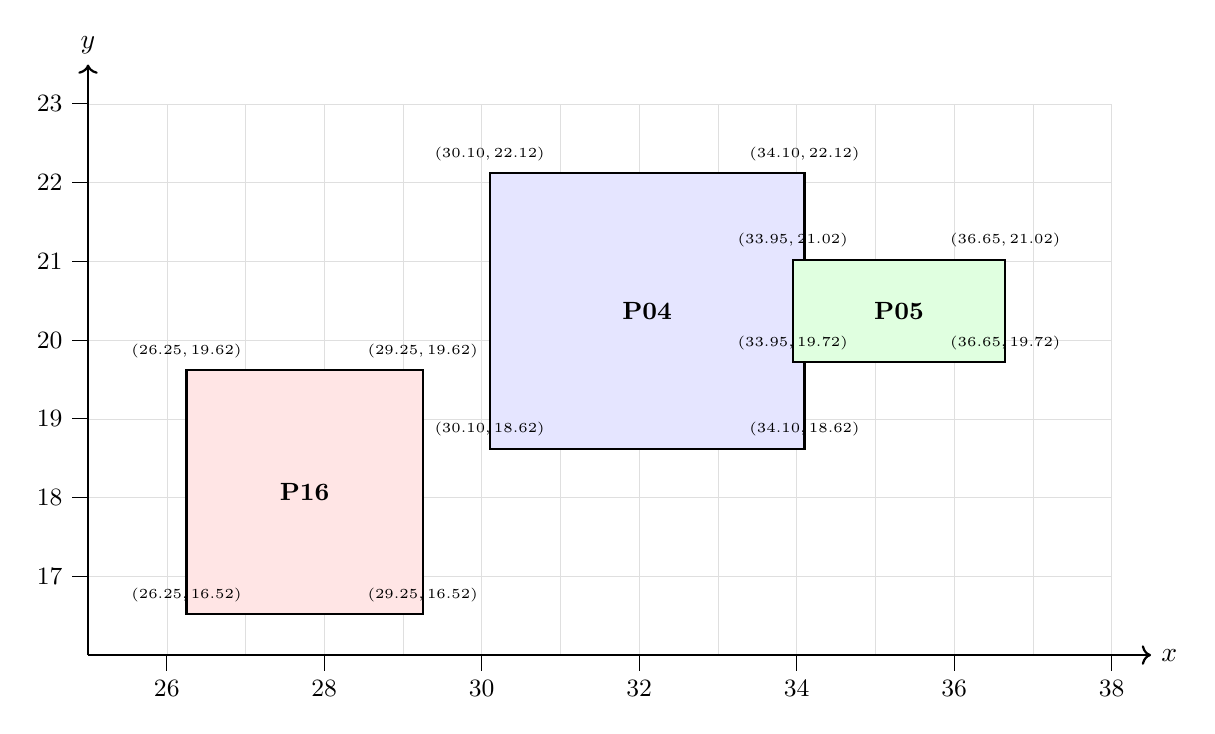
\begin{tikzpicture}[scale=1]
    
    % --------------------
    % Grade e eixos
    % --------------------
    \draw[step=1cm, gray!25, very thin] (25,16) grid (38,23);
    
    \draw[->, thick] (25,16) -- (38.5,16) node[right] {$x$};
    \draw[->, thick] (25,16) -- (25,23.5) node[above] {$y$};
    
    % Numeração dos eixos
    \foreach \x in {26,28,30,32,34,36,38}
        \draw (\x,16) -- (\x,15.8) node[below] {\small \x};
    
    \foreach \y in {17,18,19,20,21,22,23}
        \draw (25,\y) -- (24.8,\y) node[left] {\small \y};
    
    % Estilo das coordenadas
    \tikzset{
        coord/.style={font=\tiny, above=1pt, align=center}
    }
    
    % --------------------
    % Sapata 1
    % --------------------
    \draw[thick, fill=blue!10]
    (30.10,18.62) --
    (34.10,18.62) --
    (34.10,22.12) --
    (30.10,22.12) -- cycle;
    
    \node at (32.10,20.37) {\small\textbf{P04}};
    
    \node[coord] at (30.10,18.62) {(30.10,\,18.62)};
    \node[coord] at (34.10,18.62) {(34.10,\,18.62)};
    \node[coord] at (34.10,22.12) {(34.10,\,22.12)};
    \node[coord] at (30.10,22.12) {(30.10,\,22.12)};
    
    % --------------------
    % Sapata 2
    % --------------------
    \draw[thick, fill=green!12]
    (33.95,19.72) --
    (36.65,19.72) --
    (36.65,21.02) --
    (33.95,21.02) -- cycle;
    
    \node at (35.30,20.37) {\small\textbf{P05}};
    
    \node[coord] at (33.95,19.72) {(33.95,\,19.72)};
    \node[coord] at (36.65,19.72) {(36.65,\,19.72)};
    \node[coord] at (36.65,21.02) {(36.65,\,21.02)};
    \node[coord] at (33.95,21.02) {(33.95,\,21.02)};
    
    % --------------------
    % Sapata 3
    % --------------------
    \draw[thick, fill=red!10]
    (26.25,16.52) --
    (29.25,16.52) --
    (29.25,19.62) --
    (26.25,19.62) -- cycle;
    
    \node at (27.75,18.07) {\small\textbf{P16}};
    
    \node[coord] at (26.25,16.52) {(26.25,\,16.52)};
    \node[coord] at (29.25,16.52) {(29.25,\,16.52)};
    \node[coord] at (29.25,19.62) {(29.25,\,19.62)};
    \node[coord] at (26.25,19.62) {(26.25,\,19.62)};
    
    \end{tikzpicture}
    \label{fig:sobreposicao_el16}
\end{figure}




\subsubsection{Geometria}
\label{subsec:geometria_s16}

Para a verificação geométrica, aplicam-se as Equações \eqref{eq:checagem_geometria_x} e \eqref{eq:checagem_geometria_y}:

\begin{equation}
g_{geometria,x} = 1 + \frac{2 \cdot 0,05 }{0,25} -  \frac{3,00}{0,25} =  -10,6 \; <0
    \label{eq:el16_checagem_geometria_x}
\end{equation}

\begin{equation}
g_{geometria,y} = 1 + \frac{2 \cdot 0,05 }{1,20} -  \frac{3,10}{1,20}  = -1,5 \; < 0
    \label{eq:el16_checagem_geometria_y}
\end{equation}

Os valores negativos obtidos para \(g_{\text{geometria},x}\) e \(g_{\text{geometria},y}\) indicam que as restrições geométricas são plenamente satisfeitas, uma vez que as dimensões da sapata excedem de forma significativa as dimensões do pilar nas duas direções analisadas. Dessa forma, não há violação das condições geométricas impostas. Os resultados da verificação geométrica nas direções $x$ e $y$ são apresentados na Tabela \ref{tab:geometria_s16}, bem como aquele que configura o pior caso.


\begin{table}[H]
\caption{Resultados da verificação de geometria.}
\label{tab:geometria_s16}
\centering
\begin{tabular}{cccc}
\toprule
\textbf{Elemento} &
$\mathbf{g_{\mathrm{geom},x}}$ & $\mathbf{g_{\mathrm{geom},y}}$ & $\mathbf{g_{\mathrm{geom}}}$ \\
\midrule
 P04 & -12,00 & -1,27 & -1.27 \\
 P05 & -9,40  & 0,00  & 0,00  \\
 P16 & -10.60 & -1.50 & -1.50 \\
\bottomrule
\end{tabular}
\end{table}

Nota-se que, para o P05, a restrição $g_{geom,y}$ igual a zero indica que a dimensão adotada chegou ao limiar da viabilidade. Contudo, não configura um descumprimento da restrição.

\subsection{O \textit{framework }FUNDAAI}

Neste trabalho, desenvolveu-se a plataforma web \textbf{FundaAI} para dimensionamento automatizado de fundações, acessível em \url{https://fundaai.streamlit.app/}. A ferramenta implementa a metodologia proposta, proporcionando uma interface prática para aplicação em projetos reais. Ela foi implementada em um ambiente \textsc{STREAMLIT} \cite{streamlit2024}, um \textit{framework Python} de código aberto que permite criar aplicativos de dados. 

A ferramenta possibilita a importação de uma planilha de dados contendo informações da planta de fundações, incluindo dados geométricos dos elementos, características geotécnicas do solo e combinações de carregamento provenientes da superestrutura, além de parâmetros adicionais definidos diretamente pelo usuário. Esses parâmetros correspondem ao cobrimento ($cob$) à resistência característica à compressão do concreto ($f_{ck}$) em MPa e às dimensões máximas e mínimas da sapata ou do conjunto de sapatas a ser dimensionado. 

Os parâmetros citados anteriormente referem-se aos parâmetros do modelo mecânico da sapata. Além disso, o usuário define o número de iterações do algoritmo a ser empregado, bem como o tamanho da população que será empregada a cada geração para a busca da solução ótima.

O funcionamento da plataforma envolve, inicialmente, a inserção da planilha de dados e dos parâmetros de dimensionamento pelo usuário. Após essa etapa, a execução do algoritmo é iniciada, realizando assim o dimensionamento geométrico dos elementos de fundação conforme descrito na Seção \ref{sec:sapata}.

Após a conclusão da rotina de cálculos e do processo de dimensionamento, a plataforma disponibiliza duas planilhas de resultados. A primeira contém as dimensões ótimas determinadas para cada elemento analisado e a segunda apresenta o conjunto completo dos valores finais das verificações efetuadas, correspondentes à solução considerada ótima.

Com o objetivo de demonstrar a operacionalidade da ferramenta \textbf{FundaAI}, esta seção descreve a interface gráfica da plataforma, detalhando suas funcionalidades e fluxo de interação. Adicionalmente, são apresentados resultados de processos de otimização ilustrativos, baseados no problema-exemplo discutido na seção anterior, que evidenciam a eficácia da abordagem proposta.

A interface da ferramenta foi estruturada de forma intuitiva, de modo a guiar o usuário ao longo das etapas necessárias para a execução do dimensionamento. A Figura \ref{fig:pag_web_inicial} apresenta a página inicial, onde pode-se definir o idioma e ver as informações necessárias para o uso, além de baixar um exemplo de arquivo de entrada.

\begin{figure}[htpb!]
    \centering
    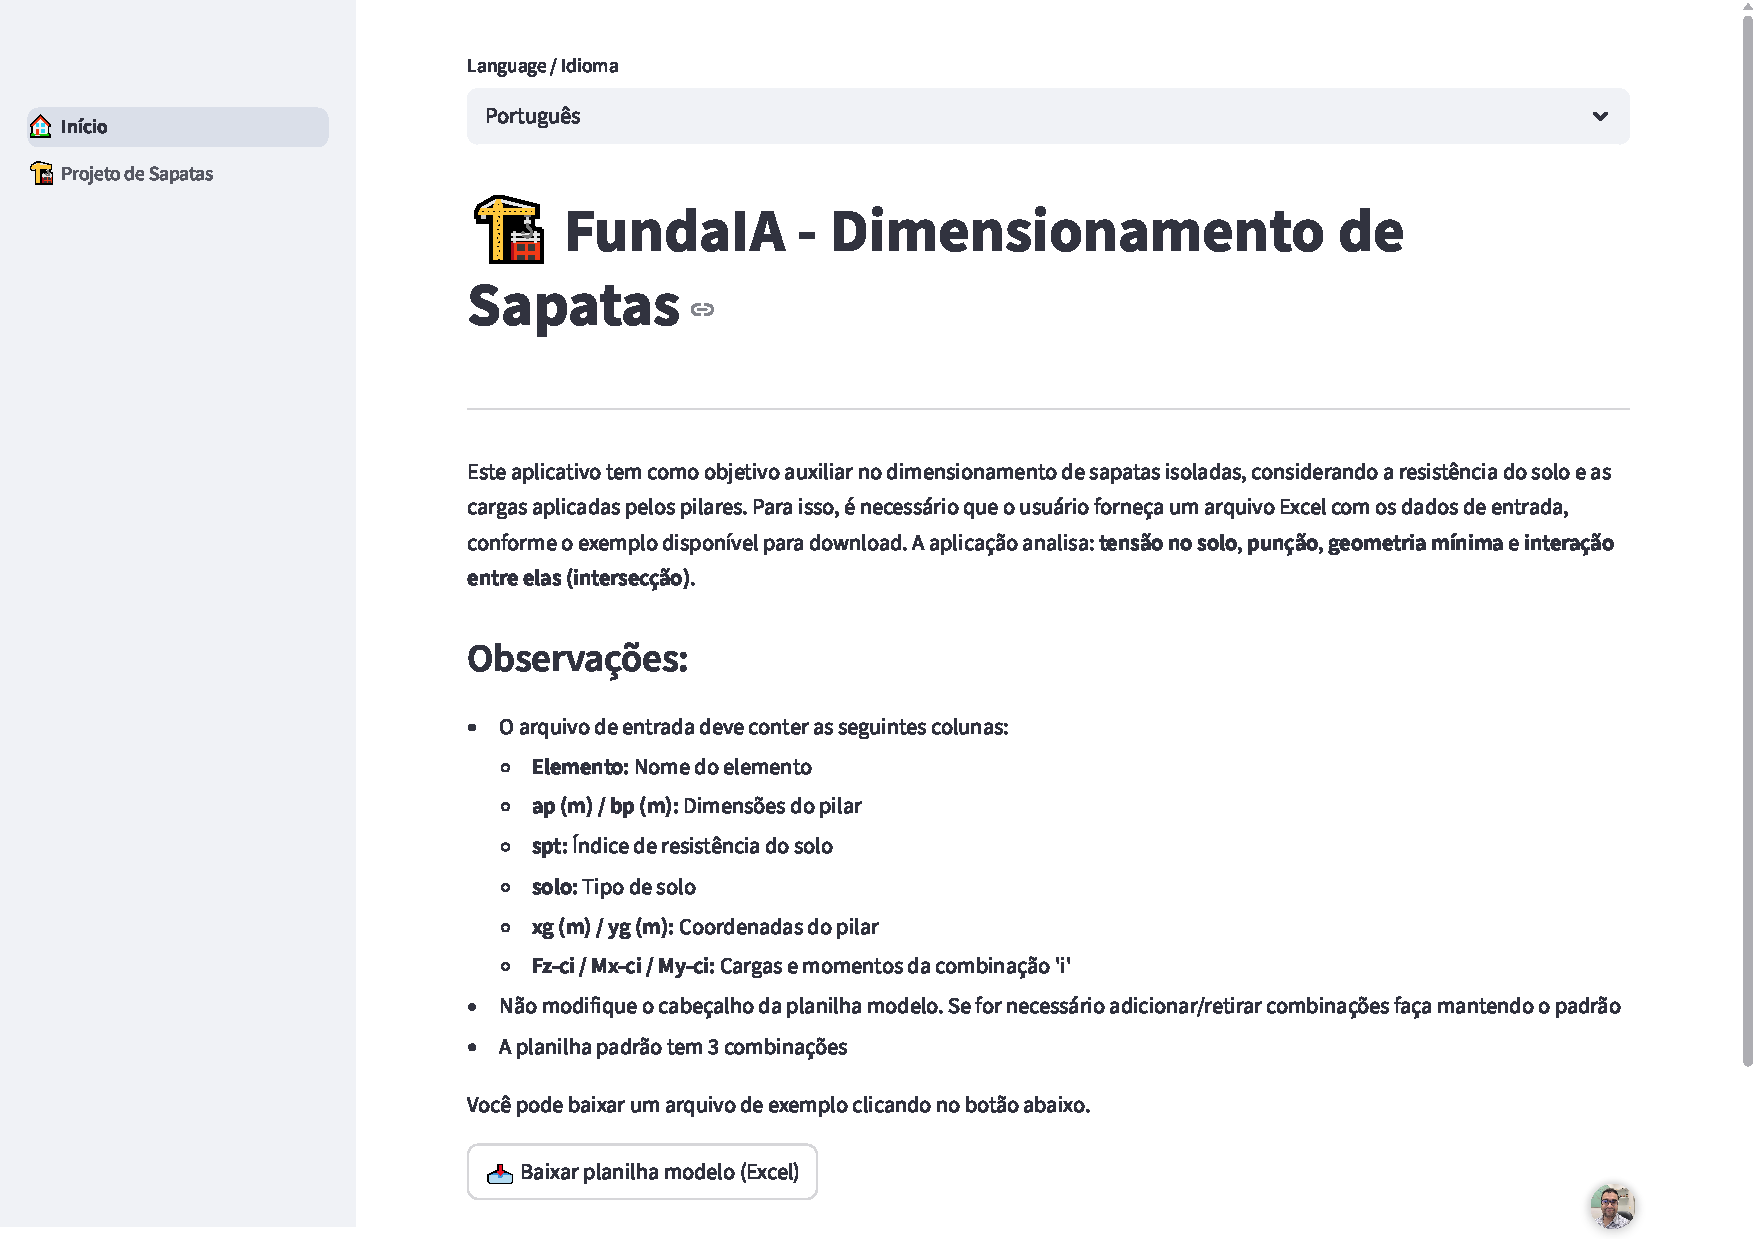
\includegraphics[width=1\linewidth]{figuras/pag_web_inicial.pdf}
    \caption{Página inicial da ferramenta \textit{web}.}
    \label{fig:pag_web_inicial}
\end{figure}

Entrando na aba "Projeto de Sapatas" (ver Figura \ref{fig:pag_web_dados}), o usuário tem acesso aos parâmetros que devem ser definidos. Na mesma aba, tem-se o local para inserção da planilha de entrada, em destaque na Figura \ref{fig:pag_web_insercao}.

\begin{figure}[htpb!]
    \centering
    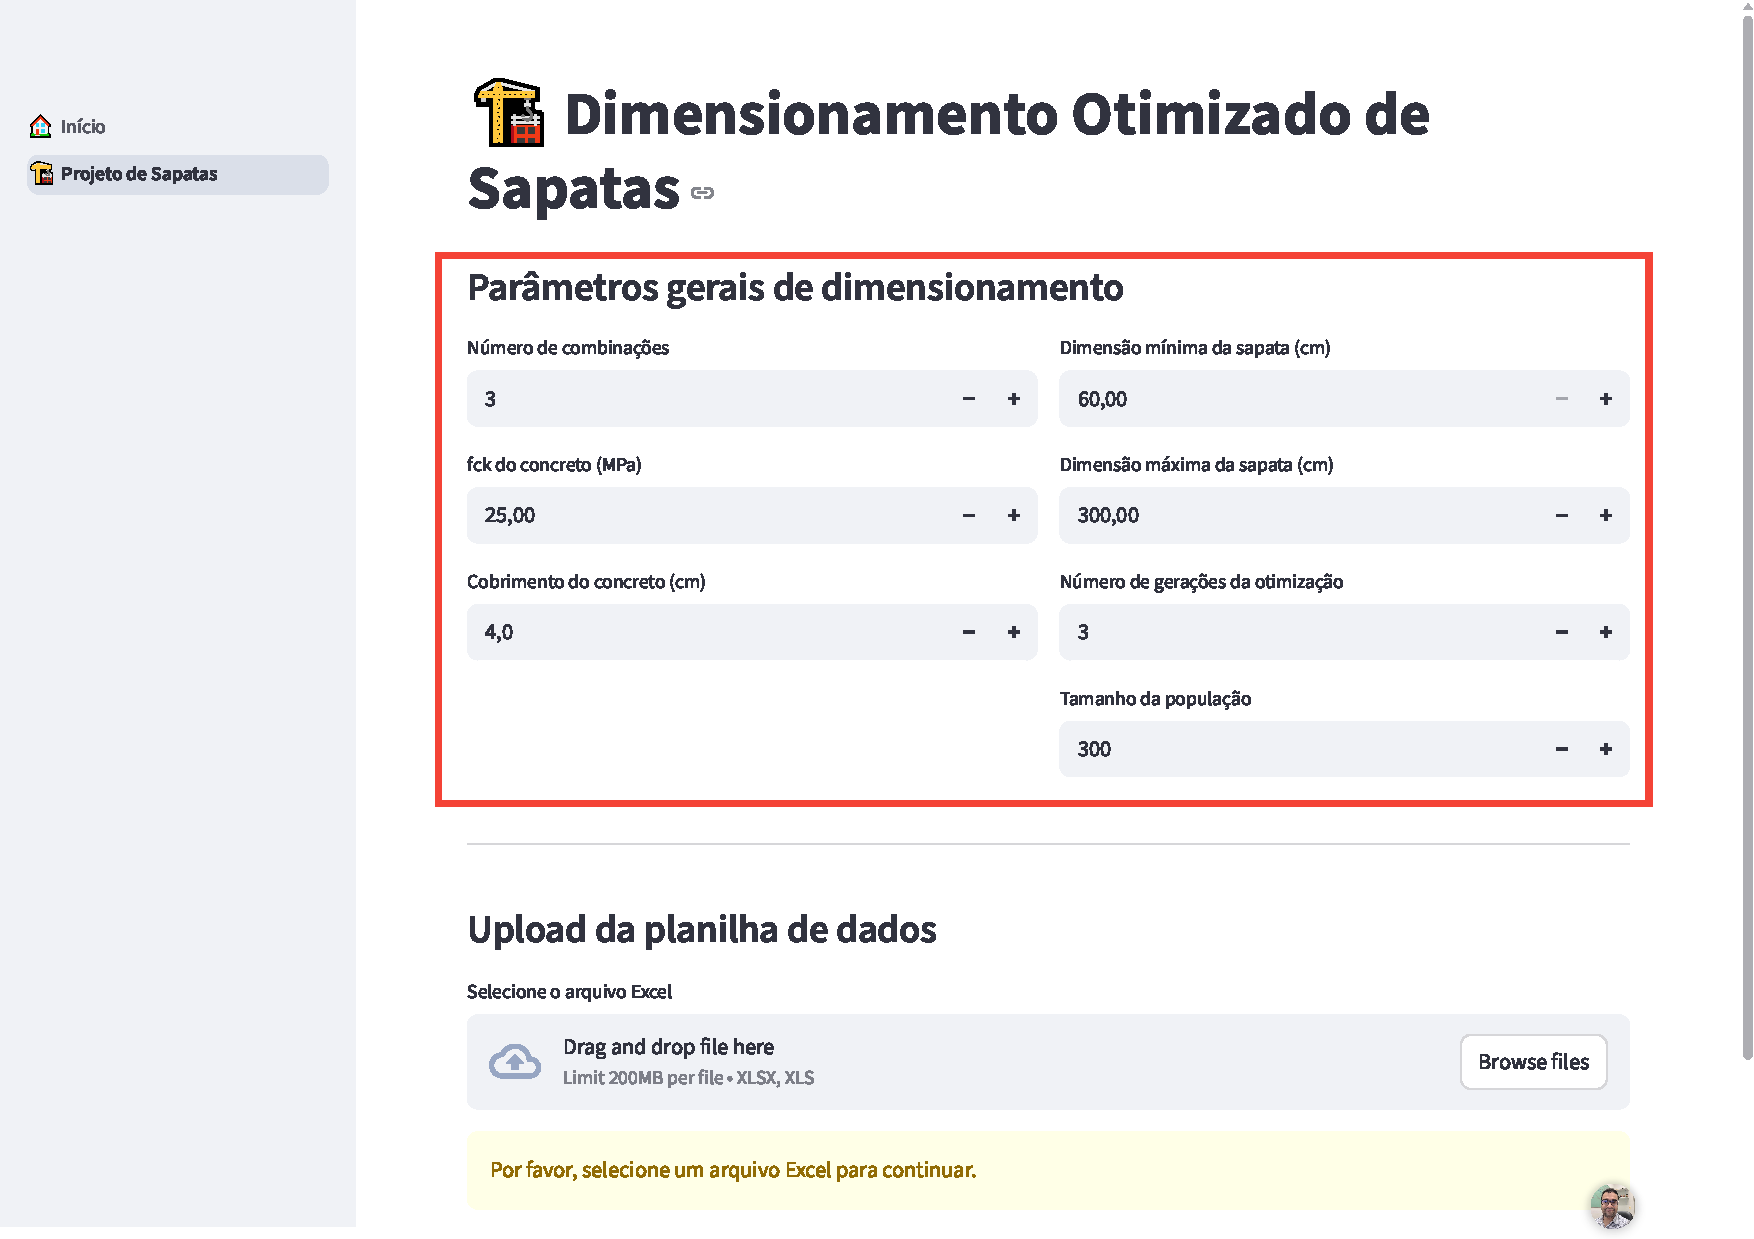
\includegraphics[width=1\linewidth]{figuras/pag_web_dados.pdf}
    \caption{Pagina de dimensionamento - Local da definição dos parâmetros.}
    \label{fig:pag_web_dados}
\end{figure}

\begin{figure}[htpb!]
    \centering
    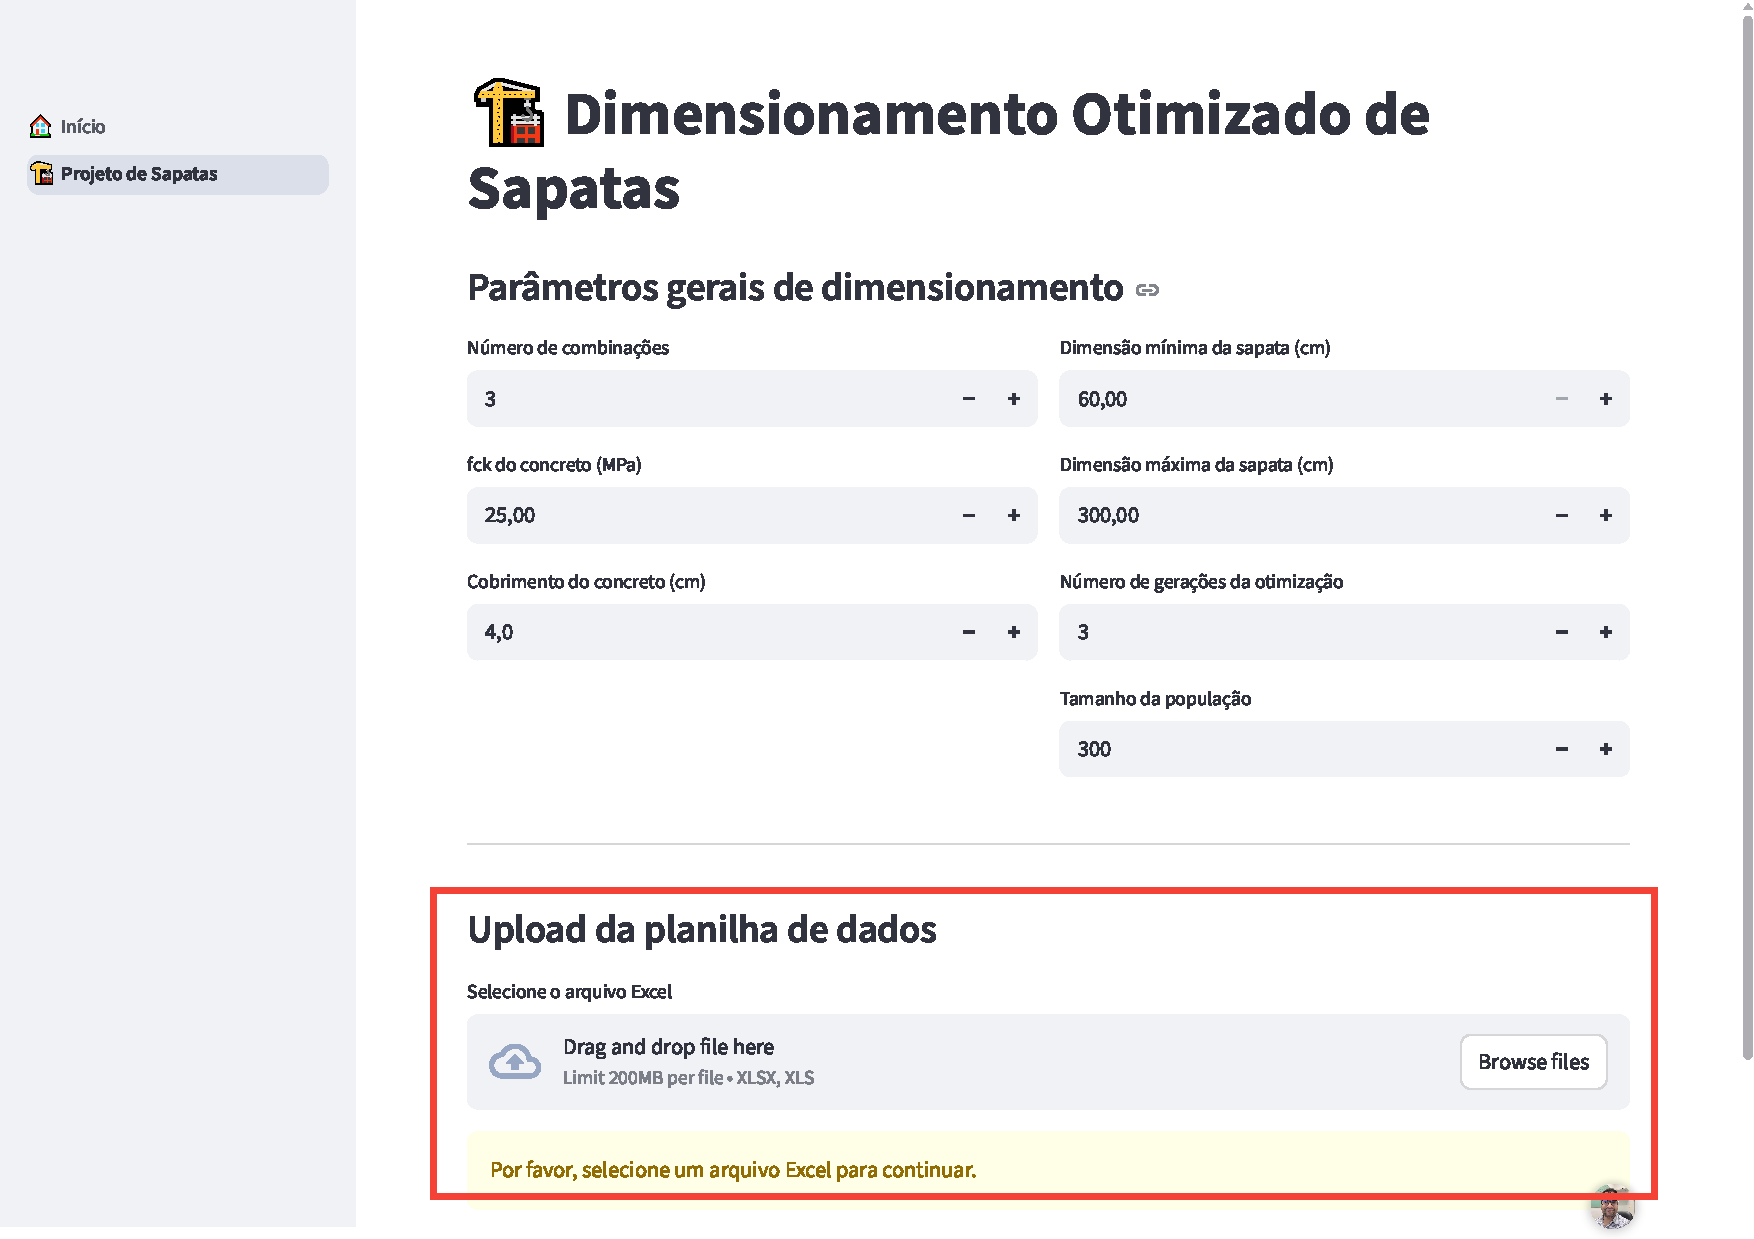
\includegraphics[width=1\linewidth]{figuras/pag_web_insercao.pdf}
    \caption{Pagina de dimensionamento - Local de inserção da planilha.}
    \label{fig:pag_web_insercao}
\end{figure}

Após a inserção dos dados de entrada, o usuário pode iniciar a execução do algoritmo por meio da interface gráfica, como aponta a Figura \ref{fig:pag_web_dimensionamento}. Durante o processamento, a ferramenta executa automaticamente as rotinas de cálculo conforme descritas ao longo deste trabalho. Ao final da execução, os resultados são apresentados ao usuário de forma organizada conforme mostra a Figura \ref{fig:pag_web_resultados} permitindo a visualização das dimensões ótimas obtidas para cada elemento de fundação e a possibilidade de baixar os resultados da rotina para os valores ótimos.

\begin{figure}[htpb!]
    \centering
    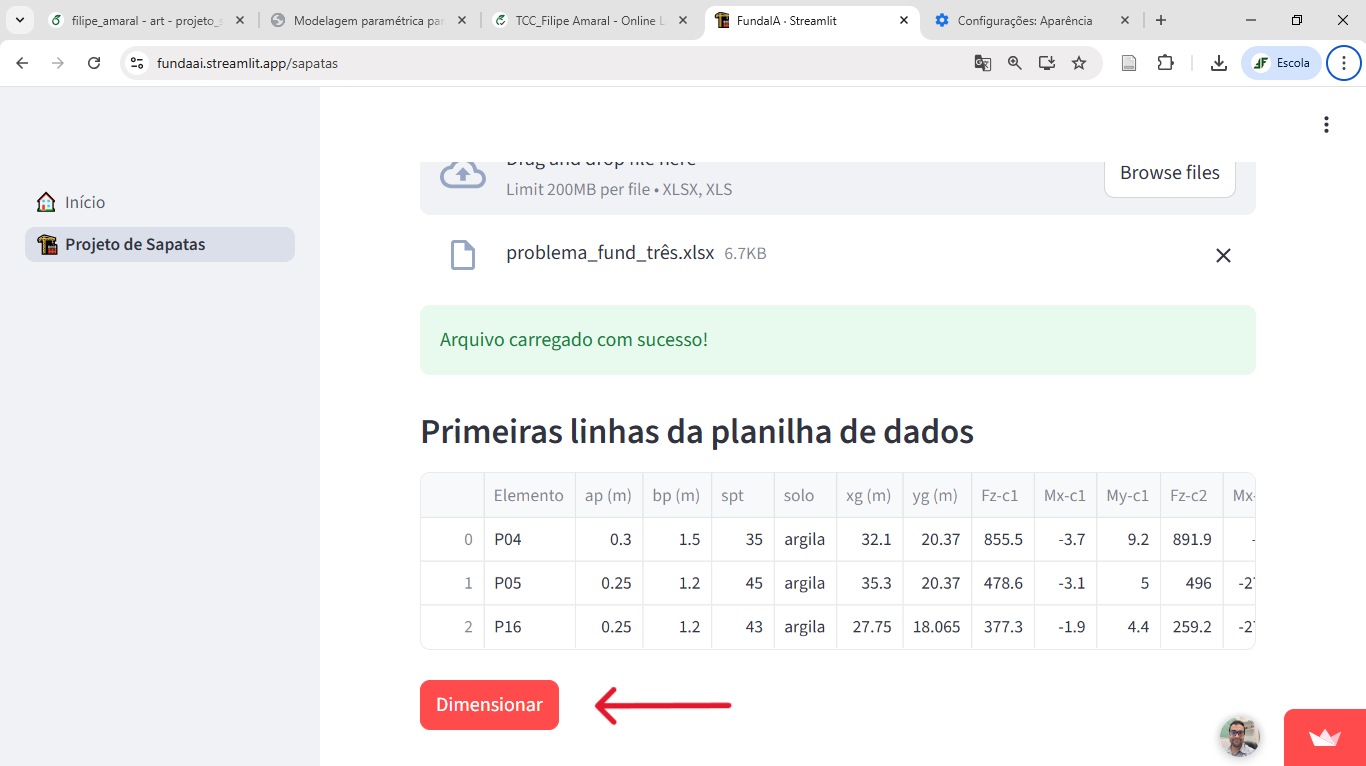
\includegraphics[width=1\linewidth]{figuras/pag_web_dimensionamento.png}
    \caption{Pagina de dimensionamento - Botão de dimensionamento.}
    \label{fig:pag_web_dimensionamento}
\end{figure}

\begin{figure}[htpb!]
    \centering
    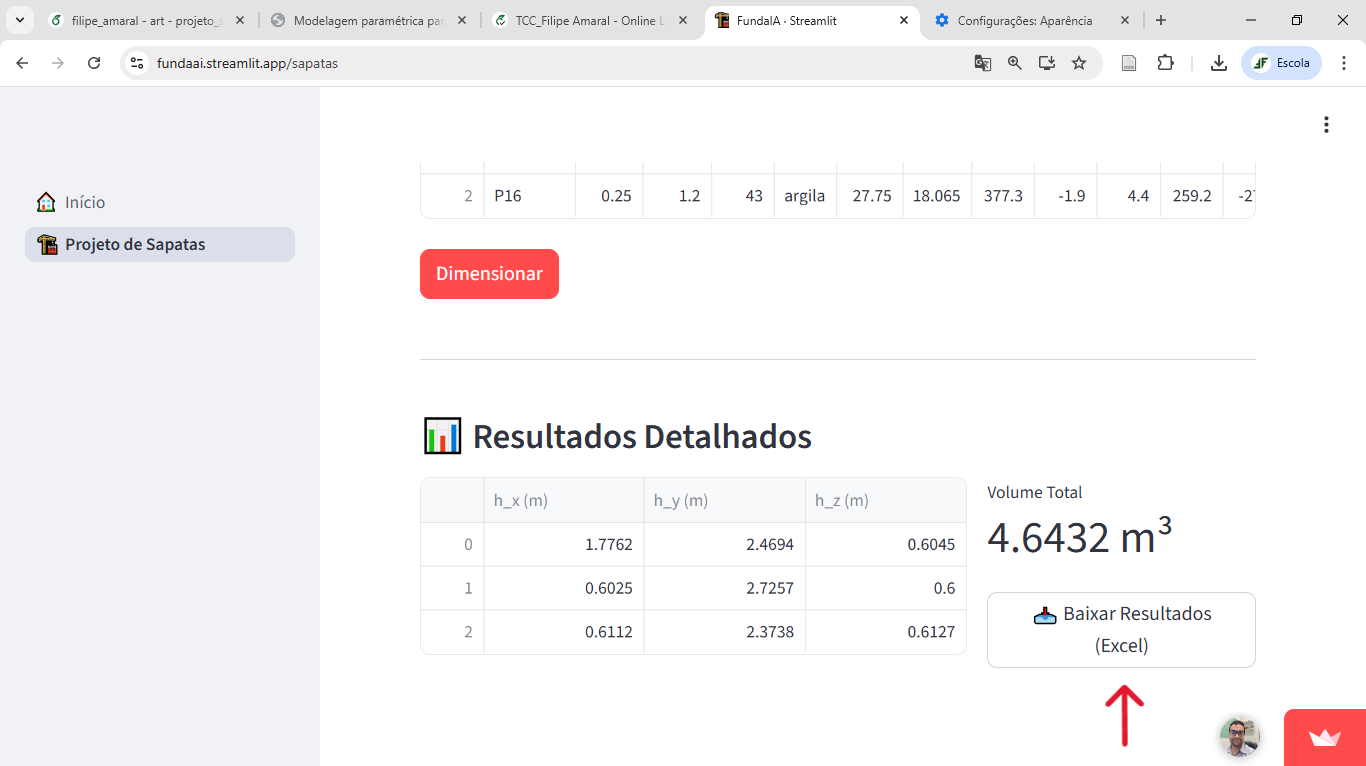
\includegraphics[width=1\linewidth]{figuras/pag_web_resultado.png}
    \caption{Pagina de dimensionamento - Resultados do dimensionamento.}
    \label{fig:pag_web_resultados}
\end{figure}


A ferramenta também disponibiliza a exportação dos resultados em formato de planilha, contendo as dimensões finais dos elementos dimensionados, juntamente com o conjunto detalhado das verificações realizadas para a solução ótima (ver Figura \ref{fig:pag_web_planilha}).  

% \begin{figure}[H]
%     \centering
%     \includegraphics[width=1\linewidth]{figuras/pag_web_planilha.png}
%     \caption{Planilha de resultados da otimização.}
%     \label{fig:pag_web_planilha}
% \end{figure}

\begin{figure}[htpb!]
    
    \centering
    \begin{subfigure}[b]{0.8\textwidth}
        \centering
        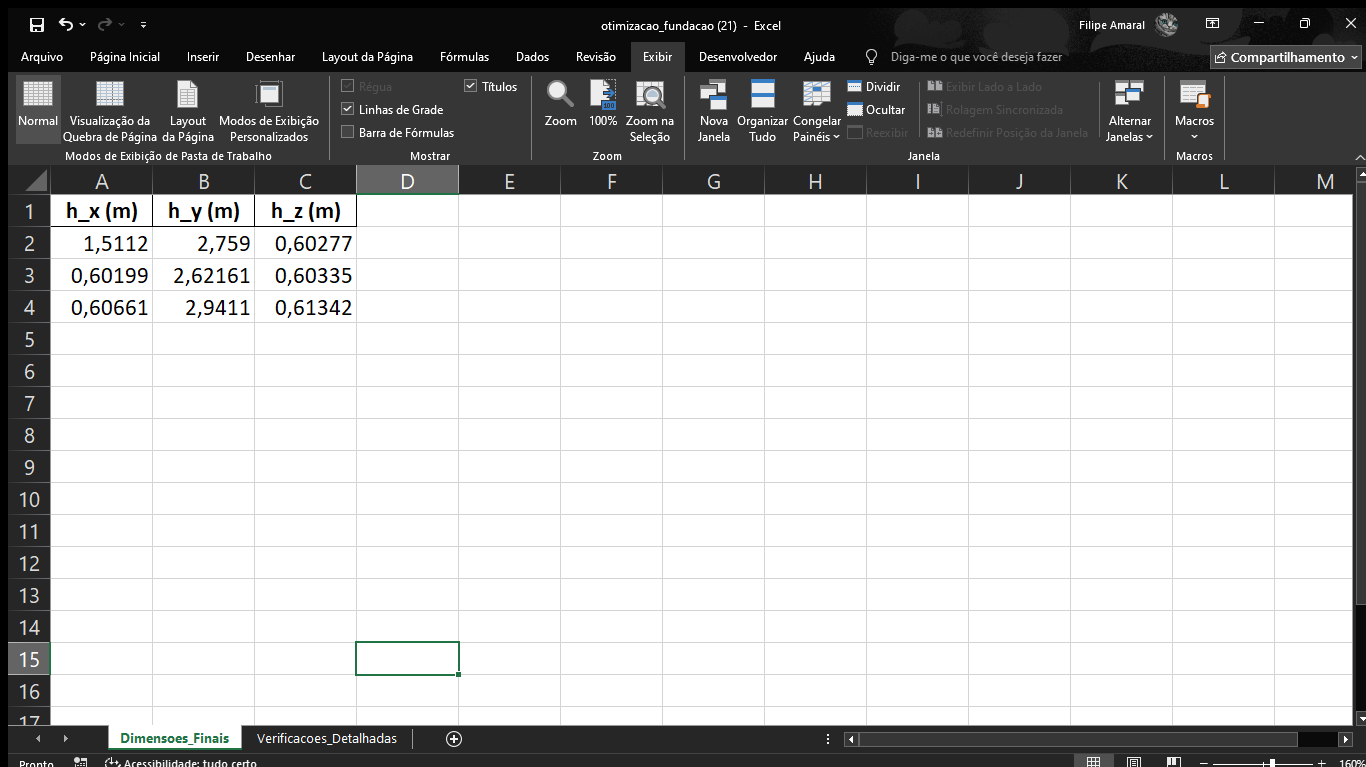
\includegraphics[width=\textwidth]{figuras/planilha a.png}
        \label{fig:exemplo_a}
    \end{subfigure}
    \hfill
    \begin{subfigure}[b]{0.8\textwidth}
        \centering
        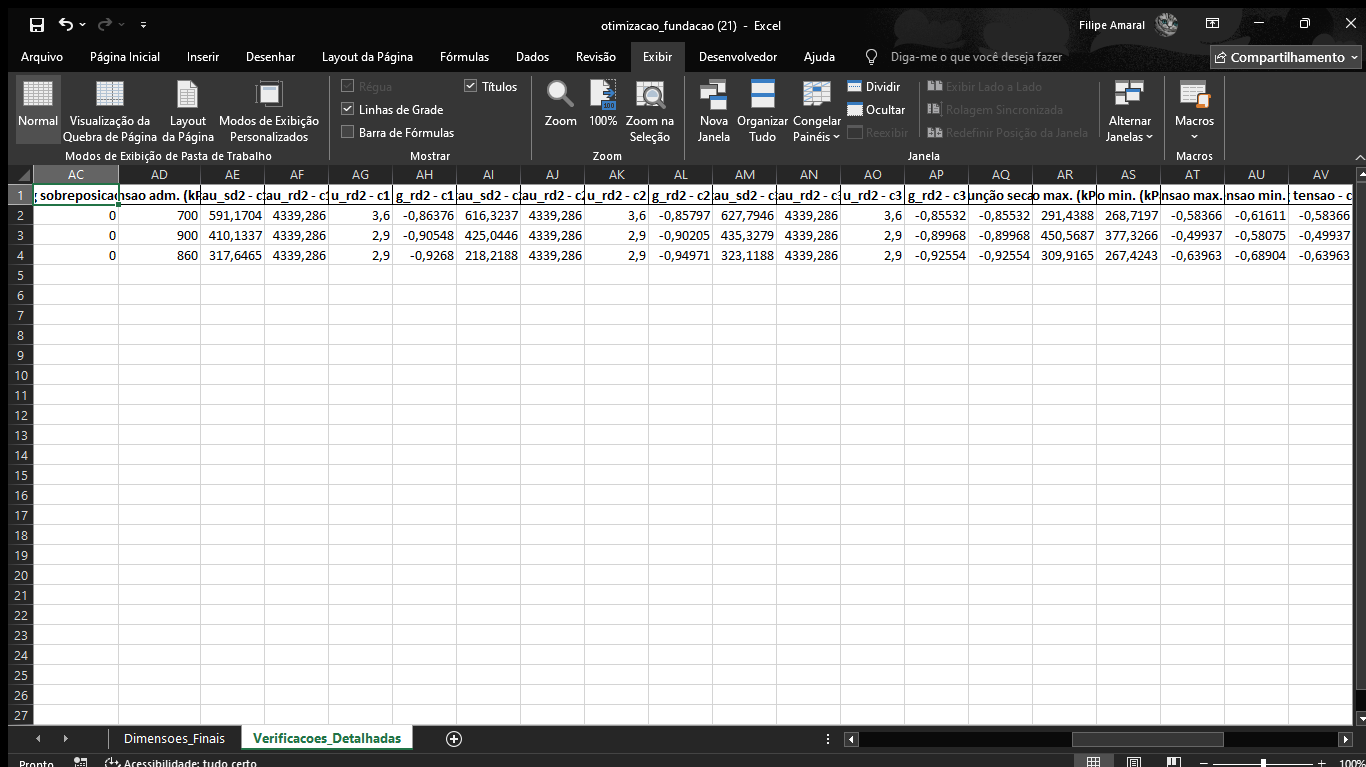
\includegraphics[width=\textwidth]{figuras/planilha b.png}

        \label{fig:exemplo_b}
    \end{subfigure}
    \caption{Planilha de resultados da otimização. (a) Dimensões ótimas e (b) Valores obtidos ao longo da verificação para as dimensões ótimas.}
    \label{fig:pag_web_planilha}
\end{figure}

\subsubsection{Resultado da otimização}

Nesta seção, são apresentados os resultados obtidos após a execução da ferramenta, ou seja, os resultados do dimensionamento otimizado. Para tanto, são empregados diferentes exemplos de projetos de fundações para demonstrar a real capacidade de uso do otimizador. Os exemplos são apresentados nas Seções seguintes, juntamente com seus respectivos resultados.

Para os processos de otimização, foi empregado o otimizador EGO (\textit{Efficient Global Optimization}), conforme descrito na Seção \ref{sec:ego}. Adotou-se uma população inicial de 300 elementos, com um número de gerações fixado em 3. O modelo substituto foi construído a partir de um processo gaussiano, no qual o \textit{kernel} foi definido de acordo com a estratégia apresentada na Seção~\ref{sec:desempenho_substituto}.

O problema de fundação consiste em um problema de 3 dimensões que correspondem as dimensões $h_x$, $h_y$ e $h_z$ da fundação. A função objetivo consiste na minimização do volume total das fundações analisadas, sendo a solução ótima definida pelo conjunto de dimensões que resulta no menor volume admissível, respeitando todas as restrições normativas e geométricas do problema. Todos esses exemplos foram executados pela interface disponível em\url{https://fundaai.streamlit.app/}.

% \paragraph{Fundação unica}
\subsubsubsection{Fundação única}

\label{item:um_elemento}

Para este exemplo utilizou-se apenas um único elemento para dimensionamento e otimização. As características do elemento estão expressas nas Tabelas \ref{tab:um_elemento} e \ref{tab:carga_um_elemento}.

\begin{table}[htbp!]
\centering
\caption{Características geométricas e do solo para o exemplo de uma fundação.}


\label{tab:um_elemento}
\setlength{\tabcolsep}{5pt}
\begin{tabular}{ c c c c c c c}
\toprule
\textbf{Elemento} &
$\mathbf{a_p \, (m)}$ &
$\mathbf{b_p \, (m)}$ &
$\mathbf{spt}$ &
$\mathbf{solo}$ &
$\mathbf{x_g \, (m)}$ &
$\mathbf{y_g \, (m)}$\\
\midrule
P08 & 2,10 & 0,25 & 12 & argila & 8,13 & 19,59 \\

\bottomrule
\end{tabular}
\end{table}

% Colocar aqui a tabela de cargas 
\begin{table}[htpb!]
\centering
\caption{Cargas atuantes para o exemplo de uma fundação.}
\label{tab:carga_um_elemento}
\setlength{\tabcolsep}{5pt}
\begin{tabular}{ c c c c c c c c c c}
\toprule
\textbf{Elemento} &
$\mathbf{F_{z,c1}}$ &
$\mathbf{M_{x,c1}}$ &
$\mathbf{M_{y,c1}}$ &
$\mathbf{F_{z,c2}}$ &
$\mathbf{M_{x,c2}}$ &
$\mathbf{M_{y,c2}}$ &
$\mathbf{F_{z,c3}}$ &
$\mathbf{M_{x,c3}}$ &
$\mathbf{M_{y,c3}}$ \\
\midrule
P08 & 857,40 & -0,20 & 115,60 & 913,00 & -0,90 & 0,10 & 950,60 & -0,90 & -0,50 \\

\bottomrule
\end{tabular}
\end{table}


Aplicando as informações na ferramenta, obtêm-se os valores otimizados: $h_x = 2,94\;m$, $h_y = 2,18\;m$, $h_z = 0,61\;m$ e $V = 3,91 \; m^3$. Os valores das restrições\footnote{ Os valores das restrições $g \le 0$ atendem aos critérios, enquanto $g > 0$ indicam desacordo. sendo que:

$g_{rd,2}^{ci}$: Restrição associada à verificação de punção na seção $C$ em função da combinação de carga $ci$; 

$g_{\sigma}^{ci}$: Restrição associada às tensões de contato entre a sapata e o solo para a combinação de carga $ci$; 

$g_{\mathrm{geom}}$: Restrição associada à compatibilidade geométrica entre o pilar e a sapata.} para o resultado encontrado, são apresentados na Tabela \ref{tab:resultado_g_uma_fundacao}.



% tabela de $g$ com a restrição mais impactante pintada de vermelho

\begin{table}[H]
\centering

\label{tab:resultado_g_uma_fundacao}
\begin{tabular}{cccccccccc}
\toprule
\textbf{Elemento} &
$\mathbf{g_{rd,2}^{c1}}$ &
$\mathbf{g_{rd,2}^{c2}}$ &
$\mathbf{g_{rd,2}^{c3}}$ &
$\mathbf{g_{\sigma}^{c1}}$ &
$\mathbf{g_{\sigma}^{c2}}$ &
$\mathbf{g_{\sigma}^{c3}}$ &
$\mathbf{g_{\mathrm{geom}}}$ \\
\midrule
 P08 & -0,90 & -0,89 & -0,89 & -0,01 & -0,19 & -0,15 & -0,07 \\
\bottomrule
\end{tabular}
\caption{Resultados das restrições para o problema de uma fundação.}
\end{table}

Considerando que a viabilidade é satisfeita ao alcançar $g \le 0$, observa-se na Tabela \ref{tab:resultado_g_uma_fundacao} que todas as restrições estruturais, geotécnicas e geométricas foram atendidas, não havendo nenhuma violação das condições impostas pelo problema. Para facilitar a interpretação dos resultados, aplicou-se a Equação \eqref{eq:solicitação/resistência}, que fornece a razão solicitação/resistência (S/R). Tal equação indica a razão de solicitação em função da resistência para as restrições que envolvem tensão, enquanto para as restrições que envolvem geometria, pode-se interpretar como valor necessário e valor permitido. Os resultados obtidos para todas as restrições são expressos na Tabela \ref{tab:S/R_uma_fundação}.


\begin{equation}
    \label{eq:solicitação/resistência}
    \frac{\text{Solicitação}}{\text{Resistência}} = \frac{Sd}{Rd} = g + 1
\end{equation}

\begin{table}[htpb!]
\centering
\caption{Razão Solicitação/Resistência (S/R) para as restrições para o problema de uma fundação.}
\label{tab:S/R_uma_fundação}
\begin{tabular}{cccccccccc}
\toprule
\textbf{Elemento} &
$\mathbf{g_{rd,2}^{c1}}$ &
$\mathbf{g_{rd,2}^{c2}}$ &
$\mathbf{g_{rd,2}^{c3}}$ &
$\mathbf{g_{\sigma}^{c1}}$ &
$\mathbf{g_{\sigma}^{c2}}$ &
$\mathbf{g_{\sigma}^{c3}}$ &
$\mathbf{g_{\mathrm{geom}}}$ \\
\midrule
P08 & 0,10	& 0,11	& 0,11	& 0,99	& 0,81	& 0,85	& 0,93 \\
\bottomrule
\end{tabular}
\end{table}

No que se refere as tensões de punção $g_{rd,2}^{c1}$, $g_{rd,2}^{c2}$ e $g_{rd,2}^{c3}$, os valores obtidos (-0,90; -0,89; -0,89) indicam elevada folga de resistência, como pode ser notado ao aplicar a Equação \eqref{eq:solicitação/resistência}, que resulta em valores na iguais a 0,10 a 0,11, ou seja, a solicitação de punção representa aproximadamente 11\% da resistência disponível. Esse comportamento evidencia que a punção não constitui a condição governante do dimensionamento, apresentando uma margem de segurança significativamente superior à necessária para a viabilidade estrutural. Além disso, os valores para cada combinação apresentaram leve variação, indicando que a variação de $F_{zk}$ surte pouca influência para essa restrição. 

Por outro lado, as restrições associadas às tensões no solo obtiveram um comportamento distinto. A combinação $g_{\sigma}^{c1}$ = -0,01 corresponde a uma razão S/R de 0,99, o que caracteriza que tal restrição teve maior impacto no processo de otimização (uma solicitação de 99\% da tensão admissível). As combinações $c2$ e $c3$, com valores de razão solicitação/resistência de 0,81 e 0,85, apresentam folgas moderadas, mas substancialmente inferiores as apreciadas na verificação à punção.

A restrição geométrica $g_{\mathrm{geom}} = -0,07$ também se encontra satisfeita, indicando o atendimento às exigências, com relativa folga, uma vez que, pela Equação \eqref{eq:solicitação/resistência}, obtém-se uma razão de 0,93, que, embora represente um valor alto, não ultrapassa a restrição de tensão. 

A analise percentual das razões S/R entre a restrição mais dominante e a menos solicitada (Equação \eqref{eq:analise_gsc1_gp_c1}) evidencia que a restrição de tensão $g_{\sigma}^{c1}$ apresenta solicitação 890\% superior à verificada para a restrição de punção $g_{rd,2}^{c1}$, a qual corresponde a mais negativa. 



\begin{equation}
    \label{eq:analise_gsc1_gp_c1}
    \frac{0,99-0,10}{0,10} \cdot 100 = 890\%
\end{equation}

Assim, conclui-se que a restrição de tensão solo-sapata $g_{\sigma}^{c1}$ é a condição governante para o processo de dimensionamento e otimização, sendo responsável por limitar o espaço de busca para as dimensões em planta.

Quando comparada às demais combinações de tensão no solo (Equações \eqref{eq:analise_gsc1_gsc2} e \eqref{eq:analise_gsc1_gsc3}), verifica-se que a combinação $c1$ impõe uma solicitação entre 16,57\% e 22,22\% superior às combinações $c2$ e $c3$, respectivamente. Esses resultados demonstram, de forma inequívoca, que a condição $g_{\sigma}^{c1}$ constitui a restrição governante do problema de otimização para essa configuração.

\begin{equation}
    \label{eq:analise_gsc1_gsc2}
    \frac{0,99-0,81}{0,81} \cdot 100 = 22,22 \%
\end{equation}

\begin{equation}
    \label{eq:analise_gsc1_gsc3}
    \frac{0,99-0,85}{0,85} \cdot 100 = 16,47\%
\end{equation}


% Executando-se o dimensionamento para  o mesmo elemento, considerando as condições de escritório, ou seja, através de tentativa e erro (foi usada uma amostragem de Monte Carlo para essa simulação, como explicitado no Item \ref{subsubsub:comparacao}), obteve-se um resultado com o volume final de 7,71 $m^3$. Para tanto, foram preparadas 200 tentativas, o que, em um escritório de engenharia, exigiria elevado esforço por parte dos profissionais e um alto grau de organização das planilhas de cálculo. E, contudo, obtiveram-se resultados menos econômicos, uma vez que o valor final foi maior que o obtido pela otimização, de 3,91 m³.

\subsubsubsection{Três elementos de fundação}
\label{item:tres_elemento}

Para este exemplo, utilizou-se um conjunto de três elementos com o intuito de dimensioná-los e otimizá-los. Tal conjunto corresponde aos elementos do problema tratado na Seção \ref{sec:problema_brinquedo} deste trabalho e, assim, suas características estão expressas nas Tabelas \ref{tab:valores_geometricos_reais} e \ref{tab:carga_atuante_real}.


Aplicando as informações na ferramenta \textit{web}, obtém-se os valores otimizados apresentados na Tabela \ref{tab:dimensoes_3_fundacoes}. Foram obtidos os valores das restrições para os resultados encontrados são apresentados na Tabela~\ref{tab:resultado_g_3_fundacoes}.

% tabela de resultado hx hy e hz

\begin{table}[H]
\centering
\caption{Dimensões finais para o problema de 3 fundações.}
\label{tab:dimensoes_3_fundacoes}
\begin{tabular}{ccccc}
\toprule
\textbf{Elemento} &
$\mathbf{h_x\,(m)}$ &
$\mathbf{h_y\,(m)}$ &
$\mathbf{h_z\,(m)}$ &
$\mathbf{V\,(m^3)}$\\
\midrule
P04 & 1,73 & 2,37 & 0,60 & 4,70\\
P05 & 0,62 & 2,72 & 0,60 & 1,01\\
P16 & 2,61 & 1,42 & 0,63 & 2,33\\
\bottomrule
\end{tabular}
\end{table}

% tabela de g com restrição mais impactante pintada de vermelho

\begin{table}[H]
\centering
\caption{Resultados das restrições para o problema de 3 fundações.}
\label{tab:resultado_g_3_fundacoes}
\begin{tabular}{ccccccccc}
\toprule
\textbf{Elemento} &
$\mathbf{g_{rd,2}^{c1}}$ &
$\mathbf{g_{rd,2}^{c2}}$ &
$\mathbf{g_{rd,2}^{c3}}$ &
$\mathbf{g_{\sigma}^{c1}}$ &
$\mathbf{g_{\sigma}^{c2}}$ &
$\mathbf{g_{\sigma}^{c3}}$ &
$\mathbf{g_{\mathrm{geom}}}$ \\
\midrule
P04 & -0,86 & -0,86 & -0,86 & -0,58 & -0,48 & -0,51 &  -0,45 \\
P05 & -0,91 & -0,90 & -0,90 & -0,54 & -0,32 & -0,31 &  -0,70 \\
P16  & -0,93 & -0,95 & -0,93 & -0,83 & -0,86 & -0,81 &  -0,01 \\
\bottomrule
\end{tabular}
\end{table}

Aplicou-se a Equação \eqref{eq:solicitação/resistência} aos valores correspondentes às restrições avaliadas, a fim de construir a Tabela \ref{tab:S/R_tres_fundação}, na qual é apresentada a razão S/R para cada verificação.

\begin{table}[htpb!]
\centering
\caption{Razão Solicitação/Resistência (S/R) para as restrições do problema de três fundações.}
\label{tab:S/R_tres_fundação}
\begin{tabular}{cccccccccc}
\toprule
\textbf{Elemento} &
$\mathbf{g_{rd,2}^{c1}}$ &
$\mathbf{g_{rd,2}^{c2}}$ &
$\mathbf{g_{rd,2}^{c3}}$ &
$\mathbf{g_{\sigma}^{c1}}$ &
$\mathbf{g_{\sigma}^{c2}}$ &
$\mathbf{g_{\sigma}^{c3}}$ &
$\mathbf{g_{\mathrm{geom}}}$ \\
\midrule
P04 & 0,14 & 0,14 & 0,14 & 0,42 & 0,52 & 0,49 & 0,55 \\
P05 & 0,09 & 0,10 & 0,10 & 0,46 & 0,68 & 0,69 & 0,30 \\
P16 & 0,07 & 0,07 & 0,05 & 0,07 & 0,17 & 0,14 & 0,99 \\
\bottomrule
\end{tabular}
\end{table}

A analise das verificações à punção ($g_{rd,2}^{c1}$, $g_{rd,2}^{c2}$ e $g_{rd,2}^{c3}$) evidencia que a razão S/R apresenta elevada folga de resistência para todas as restrições, com valores compreendidos entre 0,05 e 0,14, ou seja, correspondendo à uma solicitação de no máximo 14\% da resistência à punção. Tal resultado indica que a punção não constitui uma condição governante do dimensionamento para esta configuração. Ademais, observa-se pequena variação das restrições entre as combinações de carregamento para um mesmo elemento, reafirmando que a variação de $F_{zk}$ exerce pouca influência sobre essa restrição ou que a dimensão $h_z$ foi suficientemente grande para amortecer os efeitos de tal variação. 

Quanto às tensões de contato com o solo, os valores para as verificações situam-se com razão S/R entre 0,07 e 0,69, correspondendo a solicitações de no máximo 69\% da capacidade de suporte do solo. Observa-se que o elemento P16 tem valores mais baixos, na faixa de 0,07 a 0,17, enquanto os elementos P04 e P05 encontram-se entre 0,42 e 0,69, indicando que, para estes últimos, o efeito geotécnico foi aproximadamente 306\% mais determinante do que para o elemento P16, conforme expresso na Equação \eqref{eq:analise_gsc3_gsc2}. Esse resultado evidencia que, para o elemento P05, com 69\% de solicitação, tem-se a restrição $g_{\sigma}^{c3}$ como a mais solicitante entre as restrições geotécnicas.

\begin{equation}
    \label{eq:analise_gsc3_gsc2}
    \frac{0,69-0,17}{0,17}\cdot100= 305,88\%
\end{equation}

Porém, diferente do problema de uma única fundação, no qual o critério geotécnico era governante no dimensionamento, observa-se que, neste arranjo com três fundações, a limitação geométrica assume um papel determinante no processo de otimização. A restrição $g_{geom}$ apresenta razões S/R iguais a 0,55, 0,30 e 0,99. Nota-se que o elemento P16 encontra-se no limite geométrico, configurando-se como a restrição governante para o arranjo.

A comparação entre a maior razão observada (0,99) e a menor razão global registrada (0,05) resulta em diferença percentual de aproximadamente 1880\%, conforme indicado na Equação \eqref{eq:analise_ggeom_gp16c3}. Tal discrepância reforça a predominância da condição geométrica no controle da solução ótima, evidenciando que o processo de minimização volumétrica conduz o elemento P16 ao limite geométrico antes que as demais verificações se tornem críticas.

\begin{equation}
    \label{eq:analise_ggeom_gp16c3}
    \frac{0,99-0,05}{0,05}\cdot100= 1880\%
\end{equation}

A análise das razões permite observar que apenas um dos três elementos teve restrição que alcançou valor próximo do limite (99\% para a restrição geométrica de P16), caracterizando-se como restrição governante. Os demais elementos (P04 e P05) apresentam margens significativas em suas verificações. Esse comportamento  demonstra que a formulação adotada conduz a uma solução ótima global, na qual nem todos os elementos atingem o limite individual. Assim, embora P04 e P05 apresentem potencial para a redução de dimensões quando analisados individualmente, tal redução pode não ser significativa para o benefício global. 

Por fim, neste arranjo com três elementos, a configuração espacial, com leve grau de proximidade, permitiu que o otimizador evitasse a existência de sobreposição, contrastando com o problema da Seção \ref{sec:problema_brinquedo} em que foi apresentada sobreposição.

\subsubsubsection{Consideração para um regime com elementos sobrepostos}
\label{item:elemento_sobreoposto}

Nesta seção é apresentada a otimização de elementos com alto grau de proximidade, com o objetivo de analisar e demonstrar o comportamento da ferramenta nessas situações específicas. As Tabelas \ref{tab:dois_elemento} e \ref{tab:carga_2_elementos} apresentam os dados iniciais para o dimensionamento.

\begin{table}[H]
\centering
\caption{Características geométricas e do solo para o exemplo de duas fundações.}
\label{tab:dois_elemento}
\setlength{\tabcolsep}{5pt}
\begin{tabular}{ c c c c c c c}
\toprule
\textbf{Elemento} &
$\mathbf{a_p \, (m)}$ &
$\mathbf{b_p \, (m)}$ &
$\mathbf{spt}$ &
$\mathbf{solo}$ &
$\mathbf{x_g \, (m)}$ &
$\mathbf{y_g \, (m)}$\\
\midrule
P01 & 0,25 & 1,20 & 10 & argila & 6,90 & 26,255 \\
P02 & 0,30 & 1,50 & 12 & argila & 7,985 & 25,105 \\
\bottomrule
\end{tabular}
\end{table}

\begin{table}[H]
\centering
\caption{Carregamentos atuantes por combinação}
\label{tab:carga_2_elementos}
\begin{tabular}{cccccccccc}
\toprule
\textbf{Elemento} &
$\mathbf{F_{z}^{c1}}$ &
$\mathbf{M_{x}^{c1}}$ &
$\mathbf{M_{y}^{c1}}$ &
$\mathbf{F_{z}^{c2}}$ &
$\mathbf{M_{x}^{c2}}$ &
$\mathbf{M_{y}^{c2}}$ &
$\mathbf{F_{z}^{c3}}$ &
$\mathbf{M_{x}^{c3}}$ &
$\mathbf{M_{y}^{c3}}$ \\
\midrule
P01 & 485,9 & -0,3 & 4,1 & 511,6 & -32,4 & -0,4 & 511,6 & -32,4 & -0,4 \\
P02 & 885,8 & -1,0 & 9,2 & 912,1 & -65,4 & 0,1  & 915,9 & -40,0 & 0,1  \\
\bottomrule
\end{tabular}
\end{table}


Aplicando as informações na ferramenta, foram obtidos os resultados expressos nas Tabelas \ref{tab:dimensoes_2_fundacoes} e \ref{tab:resultado_g_2_fundacoes}.

\begin{table}[H]
\centering
\caption{Dimensões finais para o problema de 2 fundações.}
\label{tab:dimensoes_2_fundacoes}
\begin{tabular}{ccccc}
\toprule
\textbf{Elemento} &
$\mathbf{h_x\,(m)}$ &
$\mathbf{h_y\,(m)}$ &
$\mathbf{h_z\,(m)}$ &
$\mathbf{V\,(m^3)}$\\
\midrule
P01 & 2,99 & 1,40 & 0,61 & 2,55\\
P02 & 3,00 & 1,90 & 0,61 &  3.48\\
\bottomrule
\end{tabular}
\end{table}




\begin{table}[H]
\centering
\caption{Resultados das restrições para o problema de 2 fundações.}
\label{tab:resultado_g_2_fundacoes}
\begin{tabular}{ccccccccccc}
\toprule
\textbf{Elemento} &
$\mathbf{g_{\textbf{sobreposição}}}$ &
$\mathbf{g_{rd,2}^{c1}}$ &
$\mathbf{g_{rd,2}^{c2}}$ &
$\mathbf{g_{rd,2}^{c3}}$ &
$\mathbf{g_{\sigma}^{c1}}$ &
$\mathbf{g_{\sigma}^{c2}}$ &
$\mathbf{g_{\sigma}^{c3}}$ &
$\mathbf{g_{\sigma}}$ &
$\mathbf{g_{\mathrm{geom}}}$ \\
\midrule
P01 & 0,23 &-0,90 &	-0,90	& -0,90 & -0,18 & -0,06 & -0,06 & -0,06 & 0,00 \\
P02 & 0,18 & -0,86 & -0,86 & -0,86 & -0,08 & 0,04 & 0,00 & 0,04 & -0,1 \\
\bottomrule
\end{tabular}
\end{table}

A análise da Tabela \ref{tab:resultado_g_2_fundacoes} evidencia que a configuração do problema com duas fundações apresentam violação da restrição de sobreposição, com valores de $g_{\text{sobreposição}}$ iguais a 0,23 e 0,18 para os elementos P01 e P02, respectivamente. Como valores positivos indicam a extrapolação do domínio viável, conclui-se que ambas as fundações não satisfazem a questão de sobreposição, indicando que as dimensões em planta interferem entre si no arranjo espacial.

Ao analisar a Tabela \ref{tab:S/R_duas_fundação}, obtida a partir da aplicação da Equação \eqref{eq:solicitação/resistência}, percebe-se que as verificações à punção estão na faixa de 10 a 14\% de solicitação da resistência estrutural, confirmando que essa restrição não exerce influência determinante no dimensionamento para esta configuração.


\begin{table}[htpb!]
\centering
\caption{Razão Solicitação/Resistência (S/R) para as restrições do problema de duas fundações.}
\label{tab:S/R_duas_fundação}
\begin{tabular}{ccccccccccc}
\toprule
\textbf{Elemento} &
$\mathbf{g_{\textbf{sobreposição}}}$ &
$\mathbf{g_{rd,2}^{c1}}$ &
$\mathbf{g_{rd,2}^{c2}}$ &
$\mathbf{g_{rd,2}^{c3}}$ &
$\mathbf{g_{\sigma}^{c1}}$ &
$\mathbf{g_{\sigma}^{c2}}$ &
$\mathbf{g_{\sigma}^{c3}}$ &
$\mathbf{g_{\mathrm{geom}}}$ \\
\midrule
P01 & 1,30 & 0,10 & 0,10 & 0,10 & 0,82 & 0,94 & 0,94 & 1,00 \\
P02 & 1,18 & 0,14 & 0,14 & 0,14 & 0,92 & 1,04 & 1,00 & 0,90\\
\bottomrule
\end{tabular}
\end{table}

Quanto às tensões de contato entre a sapata e o solo, observa-se que o elemento P02 apresenta um valor positivo para a combinação $c2$, com $g_{\sigma}^{c2}$ igual a 0,04, o que corresponde uma uma razão S/R de 1,04, assim caracterizando uma violação da tensão admissível, com uma solicitação de 104\% da tensão resistente. As demais verificações de tensão permanecem no domínio viável, com razões S/R entre 0,82 e 1,00, indicando que algumas combinações encontram-se próximas do limite, bem como no limiar da viabilidade, embora não tenham ultrapassado.

Além disso, observa-se que a verificação de geometria apresenta valores de razão S/R na ordem de 0,90 e 1,00, evidenciando que os elementos estão próximos do limite dimensional permitido. Tal comportamento indica que o processo de otimização conduziu as dimensões em planta a valores limítrofes.

Constata-se que, devido ao alto grau de sobreposição entre os elementos, o otimizador reduziu progressivamente as dimensões, aproximando-as do limite geométrico admissível.  Entretanto, essa redução implicou no aumento das tensões de contato no solo, culminando na violação observada para o elemento P02. Ainda assim, mesmo com a diminuição das dimensões, a solução obtida não foi suficiente para eliminar completamente a sobreposição, evidenciando um conflito entre as restrições espaciais e geotécnicas na configuração analisada.

Por fim, observa-se que a ferramenta é capaz de identificar a ocorrência de sobreposição entre os elementos de fundação e de buscar alternativas para mitigar essa condição ao longo do processo de otimização. Contudo, devido ao alto grau de sobreposição, a estratégia de alterar as dimensões da sapata não foi suficiente para contornar os efeitos severos da sobreposição. Porém, ao explorar resultados que convergem nas outras restrições, a ferramenta possui potencial para questões de pré dimensionamento.


\subsubsection{Comparação de resultados obtidos por força bruta}
\label{subsubsub:comparacao}

Realizou-se o dimensionamento dos mesmos elementos aplicados nas Seções \ref{item:um_elemento}, \ref{item:tres_elemento} e \ref{item:elemento_sobreoposto}, seguindo o método de Monte Carlo (MMC), com o objetivo de reproduzir resultados equivalentes àqueles usualmente obtidos na prática de escritório. Tal prática caracteriza-se pela adoção de procedimentos iterativos baseados em tentativa e erro, nos quais sucessivas combinações de parâmetros são avaliadas até que se obtenham soluções admissíveis segundo os critérios de projeto.

Para alcançar soluções admissíveis pelo MMC foram necessárias 200 tentativas. Em um contexto profissional não necessita-se de tal volume de iterações. Contudo, ainda demandaria elevado esforço técnico, um significativo dispêndio de tempo e um alto grau de organização das planilhas de cálculo. Mesmo diante desse volume de trabalho, o resultado obtido mostrou-se pouco econômico quando comparado aos resultados produzidos pela metodologia de otimização. Ademais, no ambiente de escritório, o tempo disponível e a carga de trabalho do profissional podem influenciar diretamente o resultado final, uma vez que o projetista pode se dar por satisfeito antes de atingir a solução mais eficiente possível. Neste sentido, a Tabela \ref{tab:volume_final} traz a comparação dos resultados obtidos pelo método Monte Carlo e pela metodologia proposta, através da aplicação  da Equação \eqref{eq:diferenca_percentual}.

\begin{equation}
    \label{eq:diferenca_percentual}
    \text{Redução percentual}\;(\%) = \frac{V_{MMC} - V_{otimizado}}{V_{MMC}} \cdot 100
\end{equation}

\begin{table}[H]
\centering
\caption{Redução dos volumes obtidos pelo metodologia proposta em relação com o método tradicional.}
\label{tab:volume_final}
\begin{tabular}{ccccc}
\toprule
\textbf{Elemento} &
$\mathbf{V_{MMC}\;(m^3)}$ &
$\mathbf{V_{otimizado}\;(m^3)}$ &
\textbf{Volume reduzido} $(\%)$ \\
\midrule
P01 & 5,34 & 2,55 & 52,25 \\
P02 & 4,04 & 3,48 & 13,86 \\
P04 & 3,82 & 4,70 &  -23,04\\
P05 &  7,15 & 1,01 &  85,87\\
P08 & 7,72 & 3,91 &  49,35 \\
P16 & 6,94 & 2,33 & 66,43 \\
\bottomrule
\end{tabular}
\end{table}

A metodologia proposta demonstra uma clara vantagem ao explorar, de forma sistemática, o espaço de soluções, reduzindo a dependência de decisões subjetivas e conduzindo a resultados significativamente mais econômicos e consistentes na maioria dos elementos, alcançando uma redução média de 40,79\%. Contudo, o elemento P04 apresentou desempenho inferior em termos de redução de volume.
\section{Conclusão}O objetivo deste trabalho foi desenvolver e avaliar uma ferramenta computacional para o dimensionamento e otimização de fundações superficiais do tipo sapata isolada, integrando critérios estruturais, geotécnicos e geométricos em um único ambiente de projeto. Para tal, foi proposta uma formulação de otimização mono-objetivo baseada na minimização do volume de concreto, empregando restrições normativas e construtivas, resolvida por meio do método \textit{Efficient Global Optimization} (EGO).

Com base nos resultados obtidos, destacam-se as seguintes conclusões:
\begin{enumerate}
    \item A formulação do problema de dimensionamento como um problema de otimização com restrições mostrou-se adequada para representar, de forma concomitante, os  critérios normativos aplicados às sapatas isoladas, incluindo verificações de tensões no solo, punção, compatibilidade geométrica entre o pilar e a sapata, além da sobreposição entre elementos de fundação.
    \item O EGO mostrou-se eficiente para problemas com dimensionalidade crescente, como no dimensionamento de múltiplas sapatas, onde cada elemento contribui com três variáveis ($h_x$, $h_y$, $h_z$).
    \item A abordagem baseada em modelo substituto garante uma busca global eficaz, como evidenciado pela superioridade frente a amostragem aleatória (Monte Carlo) em termos de qualidade da solução final, validando sua capacidade de evitar convergência prematura para ótimos locais.
    \item Os exemplos analisados demonstraram que a metodologia proposta é capaz de convergir para soluções geometricamente proporcionais e tecnicamente viáveis, atendendo simultaneamente às restrições estruturais, geotécnicas e geométricas, além de apresentar uma média de redução de 40,79\%, até 85,87\%, do consumo de concreto quando comparada a abordagem MMC que representa a técnica de escritório baseada em tentativas sucessivas.
    \item A verificação explícita de sobreposição entre sapatas mostrou-se um diferencial relevante do modelo, permitindo identificar interferências geométricas em planta e incorporá-las diretamente ao processo de otimização por meio das funções de restrição normalizadas.
    \item Nos casos em que os elementos de fundação apresentam elevado grau de proximidade, os resultados indicaram que a estratégia adotada, baseada apenas na variação das dimensões das sapatas, pode conduzir a soluções que não convergem para a solução ótima do problema. Isso evidencia que a metodologia, em sua forma atual, é mais adequada a arranjos de fundações sem sobreposição severa. Dessa forma, a sobreposição poderia ser resolvida com a implementação de uma segunda etapa de otimização, na qual a associação das sapatas deve ser verificada.
    \item A implementação da metodologia em uma plataforma computacional com interface \textit{web} demonstrou a viabilidade prática da abordagem, permitindo a aplicação direta do modelo em problemas reais de projeto, com entrada de dados via planilha e exportação automatizada dos resultados de dimensionamento e verificação.
    \item Em casos com mais de um elemento de fundação, a otimização global do problema não exige que todas as fundações apresentem restrições ativas. Sob a perspectiva de projeto individual, é desejável que cada elemento opere próximo a pelo menos um estado limite, garantindo o aproveitamento eficiente de material e racionalidade construtiva.
   
\end{enumerate}

De modo geral, a metodologia proposta mostrou-se uma ferramenta eficiente e promissora para o projeto racional e automatizado de sapatas isoladas, contribuindo para a padronização do processo de dimensionamento, a redução da subjetividade do projetista e o uso mais eficiente de materiais. Como trabalhos futuros, recomenda-se a incorporação de abordagens probabilísticas e de análise de confiabilidade, a consideração de sapatas associadas em situações de elevada proximidade entre pilares e a ampliação do modelo para incluir efeitos de recalque, interação solo-estrutura e detalhamento estrutural, de modo a expandir o campo de aplicação da ferramenta desenvolvida.
    







% The aim of this paper was to evaluate the reliability index of reinforced concrete beams affected by carbonation-induced corrosion. Reinforced concrete sections with a compressive strength of 25 MPa, subjected to a class C4 environment, were analyzed. The principal conclusions are as follows:
% \begin{enumerate}
%     \item In this environmental condition, the depassivation of the reinforcement due to carbonation occurred after a period of 39 years, with a standard deviation of 18 years. This suggests that, adopting a 95\% confidence interval, the carbonation corrosion process can potentially initiate after only 3.7 years.
%     \item The longitudinal reinforcement rate influenced the period in which the target reliability index of 3.8 proposed by the JCCS [36] and the Model Code 2010 [32] for the Ultimate Limit State was reached. Adopting a concrete cover of 2.5 cm, beams with a longitudinal reinforcement ratio of 0.2\% reached this target reliability index after 60 years. However, in beams with a longitudinal reinforcement ratio of 0.9\%, this target reliability index was reached after a period of only 30 years.
%     \item A 12\% variation in the target reliability index at the Ultimate Limit State after 50 years was observed when the concrete cover was varied between 2 and 3 cm. A concrete cover of only 2 cm can result in an average reliability index of 3.28, or 2.77 if a 95\% confidence level is adopted. On the other hand, a concrete cover of 3 cm yields an average reliability index of 3.66, or up to 3.25 if a 95\% confidence level is assumed. This demonstrates the importance of increasing the concrete cover to achieve higher reliability indices. A concrete cover value of 3 cm would appear to be sufficient for structures subjected to environmental exposure class C4 to ensure that the target reliability index of 3.8 is met for the majority of structures.
%     \item Considering 3 cm of concrete cover and age over 75 years, the average reliability index value was below the minimum limit of 3.1 recommended in the design standards for the Ultimate Limit State. This indicates that an increase in the longitudinal reinforcement cover is necessary to ensure that the minimum value of 3.1 is met after 50 years.
%     \item \textcolor{red}{Based on the significant correlation depicted in Figure 5.3, a predictive model was developed to assess the structural reliability of concrete beams subjected to corrosive conditions. The resulting expression, presented as Equation (5.1), constitutes a reliable tool for evaluating the safety of concrete elements in corrosion-prone environments and is suitable for rapid condition assessments during field inspections.}
%     \item \textcolor{red}{The technique proposed in this paper has proven to be an effective method for assessing the reliability index in the Ultimate Limit State, making it a valuable tool for evaluating the long-term maintenance needs of structures. It enables the estimation of the initiation time of corrosion due to carbonation and provides the corresponding reliability index, helping in decision-making regarding when interventions are necessary to restore the target safety levels specified in design guidelines. The results indicate a reduction in the reliability index over time, especially within the first 50 years, highlighting the importance of timely maintenance to maintain structural safety. Moreover, considering the growing impact of extreme climatic conditions, there is an increasing need to reassess the partial coefficients used in design. These coefficients may need adjustment to better reflect the accelerated degradation caused by changing environmental factors, ensuring that structural safety is accurately accounted for in the face of evolving climate conditions.}
%     \item \textcolor{red}{The proposed model presents some simplifications that should be acknowledged. In particular, the analysis does not consider the reduction of steel strength caused by corrosion, nor the potential loss of concrete cross-section due to spalling as corrosion progresses. These assumptions may lead to conservative or optimistic outcomes depending on the specific structural and environmental conditions.}
%     \item \textcolor{red}{In addition, the results are valid for exposed concrete structures (without painting or protective coating), under the same environmental exposure conditions considered in the analysis. Therefore, the findings should not be generalized to different exposure scenarios without further adjustments.}    
    
% \end{enumerate}

% \textcolor{red}{The proposed methodology offers valuable insights for concrete structures and supports decision-making processes for the maintenance and life-cycle management of civil infrastructure. Furthermore, it is instrumental in prioritizing structures for detailed investigation and intervention, particularly within large asset inventories, thereby facilitating strategic resource allocation for optimized maintenance planning.} However, it should be noted that the results presented in this paper were obtained based on the humidity and temperature conditions presented in the methodology. They may differ under other climatic conditions, and the proposed predictive equation should be adjusted accordingly.




\section*{Declarações}
\subsection*{Financiamento}
Os autores agradecem o financiamento deste projeto de pesquisa pelo CAPES (processo nº 88887.110529/2025-00).

\subsection*{Conflitos de interesse}
Os autores declaram não possuir quaisquer interesses financeiros ou relações pessoais conhecidas que possam ter influenciado o trabalho relatado neste artigo.

\subsection*{Disponibilidade dos dados}
As informações necessárias para a reprodução dos resultados apresentados estão disponíveis no próprio artigo. O software desenvolvido internamente e utilizado pelos autores será disponibilizado pelo autor correspondente, wmpjr, mediante solicitação justificada.



% \subsection*{Funding}
% The authors acknowledge funding of this research project by CNPq (grant nº 305622/2023-4).

% \subsection*{Conflicts of interest}
% The authors declare that they have no known competing financial interests or personal relationships that could have appeared to influence the work reported in this paper.

% \subsection*{Data Availability}
% Information required to reproduce results shown herein is  provided in the paper. The in-house  software employed by the authors will be provided by the corresponding author, wmpjr, upon reasonable request.

\section*{Apêndice A. Problema de brinquedo}\label{apendix}
\textcolor{red}{Não apagar, pois tem formulações referente à punção no perímetro C', que pode ser necessário resgatar.!!!}
%Não apagar!!!!!!!!!
% Para o perímetro $C'$, procedem-se às verificações de punção conforme descrito a seguir. inicialmente, pela equação \eqref{eq:secao_critica_c'} é determinada a distância da seção crítica em relação ao  pilar: 

% \begin{equation}
% sc = \frac{1,00}{2} = 0,50\;m
%     \label{eq:EL16_secao_critica}
% \end{equation}

% Em seguida, com base na equação~\eqref{eq:ke}, define-se o coeficiente de escala para punção:

% \begin{equation}
% k_e = 1 + \sqrt{\frac{20}{0,96 \cdot 100}} = 1,46
% \label{eq:EL16_ke}
% \end{equation}

% \textcolor{red}{pegar essa informação com o professor}
% Para os valores da taxa de armadura, aplica-se a tabela ??? da NBR 6118, que relaciona a taxa de armadura com a resistência característica do concreto. Ao utilizar $f_{ck}$ = 25 MPa, obtem-se os valores de $rho_x = 0,15$ e $rho_y = 0,15$. Assim, de acordo com a equação \eqref{eq:rho}, tem-se:

% \begin{equation}
% rho = \frac{\sqrt{0,15 * 0,15}}{100} = 1,50 \cdot 10^{-3}
%     \label{eq:rho_el16}
% \end{equation}

% A tensão resistente à punção no perímetro $C'$ é definida por meio equação~\eqref{eq:Tensão_resistente_C'}:

% \begin{equation}
%  \tau_{rd,1} = 1000 \cdot \left(0,13 \cdot 1,46\cdot \left( 100 \cdot 1,50\cdot10^{-3} \cdot 25,00 \right) ^{\frac{1}{3}}  + 0,1 \cdot 0,00 \right) = 292,85\;kPa
%  \label{eq:EL16_Tensão_resistente_C'}
% \end{equation}

% O perímetro crítico associado a seção crítica $C'$ é definido pela equação \eqref{eq:perímetro_c'}:

% \begin{equation}
% u_{rd,1} = 2 \cdot \left( 0,25 + 1,20 \right) + 4 \pi \cdot 0,50 = 9,18\;m 
%     \label{eq:EL16_perímetro_c'}
% \end{equation}

% Os valores dos coeficientes $k_x$ e $k_y$, que fornecem a parcela do momento transmitida ao pilar por cisalhamento, são obtidos a partir da tabela 19.2 da NBR 6118, através da relação das dimensões dos pilares. Dessa forma, aplicando as equações \eqref{eq:c1-C2} e \eqref{eq:C2-C1}, tem-se:

% \begin{equation}
% C1\_C2 = \frac{0,25}{1,20} = 0,21
%     \label{eq:EL16_c1-C2}
% \end{equation}

% \begin{equation}
% C2\_C1 = \frac{1,20}{0,25} = 4,80
%     \label{eq:EL16_C2-C1}
% \end{equation}

% Após a analise da referida tabela, definem-se os coeficientes em: $k_x = 0,45$  e $k_y = 0,80$.


% Os módulos de resistência plásticos associados às direções $x$ e $y$ são calculados 
% por meio das equações \eqref{eq:wpx} e \eqref{eq:wpy}:

% \begin{equation}
% w_{px} = \frac{0,25^2}{2} + 0,25\cdot 1,20 + 4 \cdot 1,20 \cdot 0,50 + 16 \cdot 0,5^2 + 2 \cdot \pi \cdot 0,25 \cdot 0,50 = 7,52 \; m^2
% \label{eq:EL16_wpy}
% \end{equation}

% \begin{equation}
% w_{py} = \frac{1,20^2}{2} + 1,20 \cdot 0,25 + 4 \cdot 0,25 \cdot 0,50 + 16 \cdot 0,50^2 + 2 \cdot \pi \cdot 1,2 \cdot 0,50 = 9,29\;m^2
%     \label{eq:EL16_wpx}
% \end{equation}

% Em posse de tais valores, define-se a tensão solicitante de punção no perímetro crítico $C'$ conforme a equação \eqref{eq:Tensão_solicitante_C'}:
 
% \begin{equation}
%  \tau_{sd,1} = \frac{1,4 \cdot 377,30}{9,18 \cdot 0,96} + \frac{1,4\cdot 0,45 \cdot (-1,90)}{7,52 \cdot 0,96} + \frac{1,4 \cdot 0,80 \cdot 4,40}{9,29 \cdot 0,96} = 60,32 \; kPa
%      \label{eq:EL16_Tensão_solicitante_C'}
% \end{equation}

% Por fim, a verificação da restrição associada à punção na seção crítica $C'$ é realizada por meio da Equação~\eqref{eq:restricao_tensao_c'}, resultando em:

% \begin{equation}
% g_{rd,1} = \frac{60,76}{292,86} - 1 = -0,79
%     \label{eq:EL16_grd1}
% \end{equation}

% Nota-se que o valor negativo de $g_{rd,1}$ indica que a condição de resistência à punção no perímetro~$C'$ é plenamente atendida.


% Concluídos os cálculos para a combinação de esforços $c1$, procede-se à repetição da análise para as demais combinações ($c2 $ e $c3$), com o objetivo de verificar as tensões solicitantes no solo e a resistência à punção. Os resultados da verificação de punção na seção crítica $C'$  são apresentados na tabela \ref{tab:puncao_secao_c_linha_p16}, enquanto aqueles referentes à seção crítica $C$ encontram-se na tabela \ref{tab:puncao_secao_c}. Os valores relacionados às tensão solicitantes no solo estão presentes na tabela \ref{tab:tensoes_solo}:

% \begin{table}[H]
% \centering
% \caption{verificação seção $C'$}
% \label{tab:puncao_secao_c_linha_p16}
% \setlength{\tabcolsep}{10pt}
% \begin{tabular}{c c c c c c c c c}
% \toprule

% Elemento & $\tau_{rd,1}$ & $u_{rd,1}$ & $k_x$ & $k_y$ & $w_{p,x}$ & $w_{p,y}$ & $\tau_{sd,1}$ & $g_{rd,1}$ \\
% \midrule
% P16 (c1) & 292,85 & 9,18 & 0,45 & 0,80 & 7,52 & 9,29 & 60,32 & -0,79 \\
% P16 (c2) & 292,85 & 9,18 & 0,45 & 0,80 & 7,52 & 9,29 & 38,15 & -0,87 \\
% P16 (c3) & 292,85 & 9,18 & 0,45 & 0,80 & 7,52 & 9,29 & 62,42 & -0,79 \\
% \bottomrule
% \end{tabular}
% \end{table}


% \begin{table}[H]
% \centering
% \caption{Verificação à punção na seção $C$}
% \label{tab:puncao_secao_c}
% \setlength{\tabcolsep}{10pt}
% \begin{tabular}{lcccccccc}
% \hline
%  Elemento & $\tau_{sd,2}$ & $\tau_{rd,2}$ & $u_{rd,2}$ & $k_e$ & $g_{e,d}$ & $g_{rd,2}$ \\
% \hline
% P16 (c1) & 186,82 & 4339,29 & 2,90 &  1,453 & -0,274 & -0,957 & \\
% P16 (c2) & 128,34 & 4339,29 & 2,90 &  1,453 & -0,274 & -0,970 &\\
% P16 (c3) & 190,03 & 4339,29 & 2,90 &  1,453 & -0,274 & -0,956 &\\
% \hline
% \end{tabular}

% \end{table}


% \begin{table}[H]
% \centering
% \caption{Verificação das tensões no solo}
% \label{tab:tensoes_solo}
% \setlength{\tabcolsep}{5pt}
% \begin{tabular}{lrrrrrrrrr}
% \hline
% El &
% $\sigma_{\max,c1}$ & $\sigma_{\min,c1}$ & $g_{c1}$ & $\sigma_{\max,c2}$ & $\sigma_{\min,c2}$ & $g_{c2}$ & $\sigma_{\max,c3}$ & $\sigma_{\min,c3}$ & $g_{c3}$\\
% \hline
% P16 & 43,99 & 41,21 & -0,934 & 35,56 & 22,97 & -0,946 & 49,63 & 37,03 & -0,925 \\
% \hline
% \end{tabular}
% \end{table}


% Após a determinação das tensões solicitantes para todas as combinações de carregamento e a avaliação dos respectivos valores de cada restrição $g$, é selecionada a combinação que representa a situação mais crítica. Essa combinação, por representar a pior situação em termos de solicitação dentre as analisadas, é utilizada para o processamento da função-objetivo.

% Neste caso, a partir da analise dos valores de $g_{rd,1}$ e $g_{rd,2}$ apresentados na tabela \ref{tab:puncao_secao_c_linha_p16} e \ref{tab:puncao_secao_c}, observa-se que a combinação $c2$ apresenta a condição mais crítica. Dessa forma, essa combinação é adotada para dar seguimento ao processo de otimização.



\bibliographystyle{model1-num-names}
\bibliography{mybibfile.bib}

\end{document}
